% Options for packages loaded elsewhere
\PassOptionsToPackage{unicode}{hyperref}
\PassOptionsToPackage{hyphens}{url}
\PassOptionsToPackage{dvipsnames,svgnames,x11names}{xcolor}
%
\documentclass[
  a4paper,
]{report}
\usepackage{amsmath,amssymb}
\usepackage{lmodern}
\usepackage{iftex}
\ifPDFTeX
  \usepackage[T1]{fontenc}
  \usepackage[utf8]{inputenc}
  \usepackage{textcomp} % provide euro and other symbols
\else % if luatex or xetex
  \usepackage{unicode-math}
  \defaultfontfeatures{Scale=MatchLowercase}
  \defaultfontfeatures[\rmfamily]{Ligatures=TeX,Scale=1}
\fi
% Use upquote if available, for straight quotes in verbatim environments
\IfFileExists{upquote.sty}{\usepackage{upquote}}{}
\IfFileExists{microtype.sty}{% use microtype if available
  \usepackage[]{microtype}
  \UseMicrotypeSet[protrusion]{basicmath} % disable protrusion for tt fonts
}{}
\makeatletter
\@ifundefined{KOMAClassName}{% if non-KOMA class
  \IfFileExists{parskip.sty}{%
    \usepackage{parskip}
  }{% else
    \setlength{\parindent}{0pt}
    \setlength{\parskip}{6pt plus 2pt minus 1pt}}
}{% if KOMA class
  \KOMAoptions{parskip=half}}
\makeatother
\usepackage{xcolor}
\IfFileExists{xurl.sty}{\usepackage{xurl}}{} % add URL line breaks if available
\IfFileExists{bookmark.sty}{\usepackage{bookmark}}{\usepackage{hyperref}}
\hypersetup{
  pdftitle={Low-Level Software Security for Compiler Developers},
  colorlinks=true,
  linkcolor={Maroon},
  filecolor={Maroon},
  citecolor={Blue},
  urlcolor={Blue},
  pdfcreator={LaTeX via pandoc}}
\urlstyle{same} % disable monospaced font for URLs
\usepackage{color}
\usepackage{fancyvrb}
\newcommand{\VerbBar}{|}
\newcommand{\VERB}{\Verb[commandchars=\\\{\}]}
\DefineVerbatimEnvironment{Highlighting}{Verbatim}{commandchars=\\\{\}}
% Add ',fontsize=\small' for more characters per line
\newenvironment{Shaded}{}{}
\newcommand{\AlertTok}[1]{\textcolor[rgb]{1.00,0.00,0.00}{\textbf{#1}}}
\newcommand{\AnnotationTok}[1]{\textcolor[rgb]{0.38,0.63,0.69}{\textbf{\textit{#1}}}}
\newcommand{\AttributeTok}[1]{\textcolor[rgb]{0.49,0.56,0.16}{#1}}
\newcommand{\BaseNTok}[1]{\textcolor[rgb]{0.25,0.63,0.44}{#1}}
\newcommand{\BuiltInTok}[1]{\textcolor[rgb]{0.00,0.50,0.00}{#1}}
\newcommand{\CharTok}[1]{\textcolor[rgb]{0.25,0.44,0.63}{#1}}
\newcommand{\CommentTok}[1]{\textcolor[rgb]{0.38,0.63,0.69}{\textit{#1}}}
\newcommand{\CommentVarTok}[1]{\textcolor[rgb]{0.38,0.63,0.69}{\textbf{\textit{#1}}}}
\newcommand{\ConstantTok}[1]{\textcolor[rgb]{0.53,0.00,0.00}{#1}}
\newcommand{\ControlFlowTok}[1]{\textcolor[rgb]{0.00,0.44,0.13}{\textbf{#1}}}
\newcommand{\DataTypeTok}[1]{\textcolor[rgb]{0.56,0.13,0.00}{#1}}
\newcommand{\DecValTok}[1]{\textcolor[rgb]{0.25,0.63,0.44}{#1}}
\newcommand{\DocumentationTok}[1]{\textcolor[rgb]{0.73,0.13,0.13}{\textit{#1}}}
\newcommand{\ErrorTok}[1]{\textcolor[rgb]{1.00,0.00,0.00}{\textbf{#1}}}
\newcommand{\ExtensionTok}[1]{#1}
\newcommand{\FloatTok}[1]{\textcolor[rgb]{0.25,0.63,0.44}{#1}}
\newcommand{\FunctionTok}[1]{\textcolor[rgb]{0.02,0.16,0.49}{#1}}
\newcommand{\ImportTok}[1]{\textcolor[rgb]{0.00,0.50,0.00}{\textbf{#1}}}
\newcommand{\InformationTok}[1]{\textcolor[rgb]{0.38,0.63,0.69}{\textbf{\textit{#1}}}}
\newcommand{\KeywordTok}[1]{\textcolor[rgb]{0.00,0.44,0.13}{\textbf{#1}}}
\newcommand{\NormalTok}[1]{#1}
\newcommand{\OperatorTok}[1]{\textcolor[rgb]{0.40,0.40,0.40}{#1}}
\newcommand{\OtherTok}[1]{\textcolor[rgb]{0.00,0.44,0.13}{#1}}
\newcommand{\PreprocessorTok}[1]{\textcolor[rgb]{0.74,0.48,0.00}{#1}}
\newcommand{\RegionMarkerTok}[1]{#1}
\newcommand{\SpecialCharTok}[1]{\textcolor[rgb]{0.25,0.44,0.63}{#1}}
\newcommand{\SpecialStringTok}[1]{\textcolor[rgb]{0.73,0.40,0.53}{#1}}
\newcommand{\StringTok}[1]{\textcolor[rgb]{0.25,0.44,0.63}{#1}}
\newcommand{\VariableTok}[1]{\textcolor[rgb]{0.10,0.09,0.49}{#1}}
\newcommand{\VerbatimStringTok}[1]{\textcolor[rgb]{0.25,0.44,0.63}{#1}}
\newcommand{\WarningTok}[1]{\textcolor[rgb]{0.38,0.63,0.69}{\textbf{\textit{#1}}}}
\usepackage{longtable,booktabs,array}
\usepackage{multirow}
\usepackage{calc} % for calculating minipage widths
% Correct order of tables after \paragraph or \subparagraph
\usepackage{etoolbox}
\makeatletter
\patchcmd\longtable{\par}{\if@noskipsec\mbox{}\fi\par}{}{}
\makeatother
% Allow footnotes in longtable head/foot
\IfFileExists{footnotehyper.sty}{\usepackage{footnotehyper}}{\usepackage{footnote}}
\makesavenoteenv{longtable}
\usepackage{graphicx}
\makeatletter
\def\maxwidth{\ifdim\Gin@nat@width>\linewidth\linewidth\else\Gin@nat@width\fi}
\def\maxheight{\ifdim\Gin@nat@height>\textheight\textheight\else\Gin@nat@height\fi}
\makeatother
% Scale images if necessary, so that they will not overflow the page
% margins by default, and it is still possible to overwrite the defaults
% using explicit options in \includegraphics[width, height, ...]{}
\setkeys{Gin}{width=\maxwidth,height=\maxheight,keepaspectratio}
% Set default figure placement to htbp
\makeatletter
\def\fps@figure{htbp}
\makeatother
\setlength{\emergencystretch}{3em} % prevent overfull lines
\providecommand{\tightlist}{%
  \setlength{\itemsep}{0pt}\setlength{\parskip}{0pt}}
\setcounter{secnumdepth}{5}
\newlength{\cslhangindent}
\setlength{\cslhangindent}{1.5em}
\newlength{\csllabelwidth}
\setlength{\csllabelwidth}{3em}
\newlength{\cslentryspacingunit} % times entry-spacing
\setlength{\cslentryspacingunit}{\parskip}
\newenvironment{CSLReferences}[2] % #1 hanging-ident, #2 entry spacing
 {% don't indent paragraphs
  \setlength{\parindent}{0pt}
  % turn on hanging indent if param 1 is 1
  \ifodd #1
  \let\oldpar\par
  \def\par{\hangindent=\cslhangindent\oldpar}
  \fi
  % set entry spacing
  \setlength{\parskip}{#2\cslentryspacingunit}
 }%
 {}
\usepackage{calc}
\newcommand{\CSLBlock}[1]{#1\hfill\break}
\newcommand{\CSLLeftMargin}[1]{\parbox[t]{\csllabelwidth}{#1}}
\newcommand{\CSLRightInline}[1]{\parbox[t]{\linewidth - \csllabelwidth}{#1}\break}
\newcommand{\CSLIndent}[1]{\hspace{\cslhangindent}#1}
\usepackage{makeidx}
\makeindex
\newcounter{TodoCounter}
\usepackage[backgroundcolor=white,linecolor=black]{todonotes}
\let\oldtodo\todo
\usepackage{bclogo}%  \bcpanchant
\newcommand{\todospan}[1]{
  \stepcounter{TodoCounter}
  \oldtodo[caption={\arabic{TodoCounter}. #1}]{\bcpanchant #1}
}
\newcommand{\tododiv}[1]{
  \stepcounter{TodoCounter}
  \oldtodo[inline,caption={\arabic{TodoCounter}. #1}]{\bcpanchant \textit{#1}}
}
\usepackage{caption}
\captionsetup[figure]{labelformat=empty}
\ifLuaTeX
  \usepackage{selnolig}  % disable illegal ligatures
\fi

\title{Low-Level Software Security for Compiler Developers}
\author{}
\date{}

\begin{document}
\maketitle

\clearpage

\vspace*{\fill}
%\includegraphics[height=2cm]{example-image}
This work is licensed under the Creative Commons Attribution 4.0 International
License. To view a copy of this license, visit
http://creativecommons.org/licenses/by/4.0/ or send a letter to Creative
Commons, PO Box 1866, Mountain View, CA 94042, USA.

  Copyright 2021-2024 Arm Limited
\href{mailto:open-source-office@arm.com}{\nolinkurl{open-source-office@arm.com}}\\
  Copyright 2023 Bill Wendling
\href{mailto:morbo@google.com}{\nolinkurl{morbo@google.com}}\\
  Copyright 2023 Lucian Popescu
\href{mailto:lucian.popescu187@gmail.com}{\nolinkurl{lucian.popescu187@gmail.com}}\\
  Copyright 2024 Anders Waldenborg
\href{mailto:anders@0x63.nu}{\nolinkurl{anders@0x63.nu}}\\

Version 0-197-g27c14a8
\clearpage

{
\hypersetup{linkcolor=}
\setcounter{tocdepth}{2}
\tableofcontents
}
\hypertarget{introduction}{%
\chapter{Introduction}\label{introduction}}

Compilers, assemblers and similar tools generate all the binary code
that processors execute. It is no surprise then that these tools play a
major role in security analysis and hardening of relevant binary code.

Often the only practical way to protect all binaries with a particular
security hardening method is to have the compiler do it. And, with
software security becoming more and more important in recent years, it
is no surprise to see an ever increasing variety of security hardening
features and mitigations against vulnerabilities implemented in
compilers. Indeed, compared to a few decades ago, today's compiler
developer is much more likely to implement security features than not.

Furthermore, with the ever-expanding range of techniques implemented,
it's very hard to gain a basic understanding of all security features
implemented in typical compilers.

This poses a practical problem: compiler developers must be able to work
on security hardening features, yet it's hard to gain a good, basic
understanding of such compiler features.

There are a lot of materials that explain individual vulnerabilities or
attack vectors. There are also lots of presentations explaining specific
exploits. But there seems to be a limited set of materials that give a
structured overview of all vulnerabilities and exploits against which a
code generator plays a role in protecting.

This book aims to provide such a structured, broad overview. It does not
necessarily go into full details, instead aiming to give a thorough
description of all relevant high-level aspects of attacks,
vulnerabilities, mitigations, and hardening techniques. For further
details, this book provides pointers to materials with more details on
specific techniques.

The purpose of this book is to serve as a guide to every compiler
developer that needs to learn about software security relevant to
compilers. Even though the focus is on compiler developers, we expect
that this book will also be useful to people working on other low-level
software.

\hypertarget{why-an-open-source-book}{%
\section{Why an open source book?}\label{why-an-open-source-book}}

The idea for this book emerged out of a frustration of not finding a
good overview on this topic. Kristof Beyls and Georgia Kouveli, both
compiler engineers working on security features, wished a book like this
would exist. After not finding such a book, they decided to try and
write one themselves. They immediately realized that they do not have
all necessary expertise themselves to complete such a daunting task. So
they decided to try and create this book in an open source style,
seeking contributions from many experts.

As you read this, the book remains unfinished. This book may well never
be finished, as new vulnerabilities continue to be discovered regularly.
Our hope is that developing the book as an open source project will
allow for it to continue to evolve and improve. The open source
development process of this book increases the likelihood that it
remains relevant as new vulnerabilities and mitigations emerge.

Kristof and Georgia, the initial authors, are far from experts on all
possible vulnerabilities. So what is the plan to get high quality
content to cover all relevant topics? It is two-fold.

First, by studying specific topics, they hope to gain enough knowledge
to write up a good summary for this book.

Second, they very much invite and welcome contributions. If you're
interested in potentially contributing content, please go to the home
location for the open source project at
\url{https://github.com/llsoftsec/llsoftsecbook}.

As this book is very much a work in progress, you will notice plenty of
``TODO'' items throughout this book. \todospan{{This is an example
``TODO'' item}}

We think that keeping the TODOs clearly visible helps both readers and
potential contributors. Readers get hints of what kind of further
content is still missing. Potential contributors get hints for where we
need help to further improve this book.

As a reader, you can also contribute to making this book better. We
highly encourage feedback, both positive and constructive criticisms. We
prefer feedback through either
\url{https://github.com/llsoftsec/llsoftsecbook}, for example by raising
an issue there, or through our
\href{https://discord.gg/Bm55Z9Ppgn}{Discord server}. Interested
potential contributors can reach the LLSoftSec community through the
same channels.

\tododiv{Add section describing the structure of the rest of the book.}

\hypertarget{memory-vulnerability-based-attacks}{%
\chapter{Memory vulnerability based
attacks}\label{memory-vulnerability-based-attacks}}

\hypertarget{a-bit-of-background-on-memory-vulnerabilities}{%
\section{A bit of background on memory
vulnerabilities}\label{a-bit-of-background-on-memory-vulnerabilities}}

Memory access errors describe memory accesses that, although permitted
by a program, were not intended by the programmer. These types of errors
are usually defined (\protect\hyperlink{ref-Hicks2014}{Hicks 2014}) by
explicitly listing their types, which include:

\begin{itemize}
\tightlist
\item
  buffer overflow
\item
  null pointer dereference
\item
  use after free
\item
  use of uninitialized memory
\item
  illegal free
\end{itemize}

Memory vulnerabilities are an important class of vulnerabilities that
arise due to these types of errors, and they most commonly occur due to
programming mistakes when using languages such as C/C++
\index{C}\index{C++}. These languages do not provide mechanisms to
protect against memory access errors by default. An attacker can exploit
such vulnerabilities to leak sensitive data or overwrite critical memory
locations and gain control of the vulnerable program.

Memory vulnerabilities have a long history. The
\href{https://en.wikipedia.org/wiki/Morris_worm}{Morris worm} in 1988
was the first widely publicized attack exploiting a buffer overflow.
Later, in the mid-90s, a few famous write-ups describing buffer
overflows appeared (\protect\hyperlink{ref-AlephOne1996}{Aleph One
1996}). \protect\hyperlink{stack-buffer-overflows}{Stack buffer
overflows} were mitigated with
\protect\hyperlink{stack-buffer-overflows}{stack canaries} and
\protect\hyperlink{stack-buffer-overflows}{non-executable stacks}. The
answer was more ingenious ways to bypass these mitigations:
\protect\hyperlink{code-reuse-attacks}{code reuse attacks}, starting
with attacks like
\protect\hyperlink{code-reuse-attacks}{return-into-libc}
(\protect\hyperlink{ref-Solar1997}{Solar Designer 1997}). Code reuse
attacks later evolved to
\protect\hyperlink{return-oriented-programming}{Return-Oriented
Programming (ROP)} (\protect\hyperlink{ref-Shacham2007}{Shacham 2007})
and even more complex techniques.

To defend against code reuse attacks, the
\protect\hyperlink{aslr}{Address Space Layout Randomization (ASLR)} and
\protect\hyperlink{cfi}{Control-Flow Integrity (CFI)} measures were
introduced. This interaction between offensive and defensive security
research has been essential to improving security, and continues to this
day. Each newly deployed mitigation results in attempts, often
successful, to bypass it, or in alternative, more complex exploitation
techniques, and even tools to automate them.

Memory safe (\protect\hyperlink{ref-Hicks2014}{Hicks 2014}) languages
are designed with prevention of such vulnerabilities in mind and use
techniques such as bounds checking and automatic memory management. If
these languages promise to eliminate memory vulnerabilities, why are we
still discussing this topic?

On the one hand, C and C++ \index{C}\index{C++} remain very popular
languages, particularly in the implementation of low-level software. On
the other hand, programs written in memory safe languages can themselves
be vulnerable to memory errors as a result of bugs in how they are
implemented, e.g.~a bug in their compiler. Can we fix the problem by
also using memory safe languages for the compiler and runtime
implementation? Even if that were as simple as it sounds, unfortunately
there are types of programming errors that these languages cannot
protect against. For example, a logical error in the implementation of a
compiler or runtime for a memory safe language can lead to a memory
access error not being detected. We will see examples of such logic
errors in compiler optimizations in a
\protect\hyperlink{jit-compiler-vulnerabilities}{later section}.

Given the rich history of memory vulnerabilities and mitigations and the
active developments in this area, compiler developers are likely to
encounter some of these issues over the course of their careers. This
chapter aims to serve as an introduction to this area. We start with a
discussion of exploitation primitives, which can be useful when
analyzing threat models \todospan{{Discuss threat models elsewhere in
book and refer to that section here
\href{https://github.com/llsoftsec/llsoftsecbook/issues/161}{\#161}}}.
We then continue with a more detailed discussion of the various types of
vulnerabilities, along with their mitigations, presented in a rough
chronological order of their appearance, and, therefore, complexity.

\hypertarget{exploitation-primitives}{%
\section{Exploitation primitives}\label{exploitation-primitives}}

Newcomers to the area of software security may find themselves lost in
many blog posts and other publications describing specific memory
vulnerabilities and how to exploit them. Two very common, yet unfamiliar
to a newcomer, terms that appear in such publications are \emph{read
primitive} and \emph{write primitive}. In order to understand memory
vulnerabilities and be able to design effective mitigations, it's
important to understand what these terms mean, how these primitives
could be obtained by an attacker, and how they can be used.

An \emph{exploit primitive}\index{exploit primitive} is a mechanism that
allows an attacker to perform a specific operation in the memory space
of the victim program. This is done by providing specially crafted input
to the victim program.

A \emph{write primitive}\index{write primitive} gives the attacker some
level of write access to the victim's memory space. The value written
and the address written to may be controlled by the attacker to various
degrees. The primitive, for example, may allow:

\begin{itemize}
\tightlist
\item
  writing a fixed value to an attacker-controlled address, or
\item
  writing to an address consisting of a fixed base and an
  attacker-controlled offset limited to a specific range (e.g.~a 32-bit
  offset)\todospan{{Consider describing in more detail why the range
  limitation
  matters\href{https://github.com/llsoftsec/llsoftsecbook/issues/162}{\#162}}},
  or
\item
  writing to an attacker-controlled base address with a fixed offset.
\end{itemize}

Primitives can be further classified according to more detailed
properties. See slide 11 of (\protect\hyperlink{ref-Miller2012}{Miller,
n.d.}) for an example.

The most powerful version of a write primitive is an \emph{arbitrary
write} primitive, where both the address and the value are fully
controlled by the attacker.

A \emph{read primitive}\index{read primitive}, respectively, gives the
attacker read access to the victim's memory space. The address of the
memory location accessed will be controlled by the attacker to some
degree, as for the write primitive. A particularly useful primitive is
an \emph{arbitrary read} primitive, in which the address is fully
controlled by the attacker.

The effects of a write primitive are perhaps easier to understand, as it
has obvious side-effects: a value is written to the victim program's
memory. But how can an attacker observe the result of a read primitive?

This depends on whether the attack is interactive or non-interactive
(\protect\hyperlink{ref-Hu2016}{Hu et al. 2016}).

\begin{itemize}
\tightlist
\item
  In an \emph{interactive attack}\index{interactive attack}, the
  attacker gives malicious input to the victim program. The malicious
  input causes the victim program to perform the read the attacker
  instructed it to, and to output the results of that read. This output
  could be any kind of output, for example a network packet that the
  victim transmits. The attacker can observe the result of the read
  primitive by looking at this output, for example parsing this network
  packet. This process then repeats: the attacker sends more malicious
  input to the victim, observes the output and prepares the next input.
  You can see an example of this type of attack in
  (\protect\hyperlink{ref-Beer2020}{Beer 2020}), which describes a
  zero-click radio proximity exploit.
\item
  In a \emph{non-interactive (one-shot)
  attack}\index{non-interactive (one-shot)
  attack}, the attacker provides all malicious input to the victim
  program at once. The malicious input triggers multiple primitives one
  after the other, and the primitives are able to observe the effects of
  the preceding operations through the victim program's state. The input
  could be, for example, in the form of a JavaScript program
  (\protect\hyperlink{ref-Grouxdf2020}{Groß 2020}), or a PDF file
  pretending to be a GIF (\protect\hyperlink{ref-Beer2021}{Beer and Groß
  2021}).
\end{itemize}

\tododiv{The references in this section describe complicated modern
exploits. Consider linking to simpler exploits, as well as some
tutorial-level material.
\href{https://github.com/llsoftsec/llsoftsecbook/issues/163}{\#163}}

How does an attacker obtain these kinds of primitives in the first
place? The details vary, and in some cases it takes a combination of
many techniques, some of which are out of scope for this book. But we
will be describing a few of them in this chapter. For example a stack
buffer overflow results in a (restricted) write primitive when the input
size exceeds what the program expected.

As part of an attack, the attacker will want to execute each primitive
more than once, since a single read or write operation will rarely be
enough to achieve their end goal (more on this later). How can
primitives be combined to perform multiple reads/writes?

In the case of an interactive attack, preparing and sending input to the
victim program and parsing the output of the victim program are usually
done in an external program that drives the exploit. The attacker is
free to use a programming language of their choice, as long as they can
interact with the victim program in it. Let's assume, for example, an
exploit program in C, communicating with the victim program over TCP. In
this case, the primitives are abstracted into C functions, which prepare
and send packets to the victim, and parse the victim's responses. Using
the primitives is then as simple as calling these functions. These calls
can be easily combined with arbitrary computations, all written in C, to
form the exploit.

For this cycle of repeated input/output interactions to work, the state
of the victim program must not be lost between the different iterations
of providing input and observing output. In other words, the victim
process must not be restarted.

It's interesting to note that while the read/write primitives consist of
carefully constructed inputs to the victim program, the attacker can
view these inputs as \emph{instructions} to the victim program. The
victim program effectively implements an interpreter unintentionally,
and the attacker can send instructions to this interpreter. This is
explored further in (\protect\hyperlink{ref-Dullien2020}{Dullien 2020}).

In the case of a non-interactive attack, all computation happens within
the victim program. The duality of input data and code is even more
obvious in this case, as the malicious input to the victim can be viewed
as the exploit code. There are cases for which the input is obviously
interpreted as code by the victim application as well, as in the case of
a JavaScript program given as input to a JavaScript engine. In this
case, the read/write primitives would be written as JavaScript
functions, which when called have the unintended side-effect of
accessing arbitrary memory that a JavaScript program is not supposed to
have access to. The primitives can be chained together with arbitrary
computations, also expressed in JavaScript.

There are, however, cases where the correspondence between data and code
isn't as obvious. For example, in (\protect\hyperlink{ref-Beer2021}{Beer
and Groß 2021}), the malicious input consists of a PDF file,
masquerading as a GIF. Due to an integer overflow bug in the PDF
decoder, the malicious input leads to an unbounded buffer access,
therefore to an arbitrary read/write primitive. In the case of
JavaScript engine exploitation, the attacker would normally be able to
use JavaScript operations and perform arbitrary computations, making
exploitation more straightforward. In this case, there are no scripting
capabilities officially supported. The attackers, however, take
advantage of the compression format intricacies to implement a small
computer architecture, in thousands of simple commands to the decoder.
In this way, they effectively \emph{introduce} scripting capabilities
and are able to express their exploit as a program to this architecture.

So far, we have described read/write primitives. We have also discussed
how an attacker might perform arbitrary computations:

\begin{itemize}
\tightlist
\item
  in an external program in the case of interactive attacks, or
\item
  by using scripting capabilities (whether originally supported or
  introduced by the attacker) in non-interactive attacks.
\end{itemize}

Assuming an attacker has gained these capabilities, how can they use
them to achieve their goals?

The ultimate goal of an attacker may vary: it may be, among other
things, getting access to a system, leaking sensitive information or
bringing down a service. Frequently, a first step towards these wider
goals is arbitrary code execution\index{arbitrary code execution} within
the victim process. We have already mentioned that the attacker will
typically have arbitrary computation capabilities at this point, but
arbitrary code execution also involves things like calling arbitrary
library functions and performing system calls.

Some examples of how the attacker may use the obtained primitives:

\begin{itemize}
\tightlist
\item
  Leak information, such as pointers to specific data structures or
  code, or the stack pointer.
\item
  Overwrite the stack contents, e.g.~to perform a
  \protect\hyperlink{rop}{ROP attack}.
\item
  Overwrite non-control data, e.g.~authorization state. Sometimes this
  step is sufficient to achieve the attacker's goal, bypassing the need
  for arbitrary code execution.
\end{itemize}

Once arbitrary code execution is achieved, the attacker may need to
exploit additional vulnerabilities in order to escape a process sandbox,
escalate privilege, etc. Such vulnerability chaining is common, but for
the purposes of this chapter we will focus on:

\begin{itemize}
\tightlist
\item
  Preventing memory vulnerabilities in the first place, thus stopping
  the attacker from obtaining powerful read/write primitives.
\item
  Mitigating the effects of read/write primitives, e.g.~with mechanisms
  to maintain \protect\hyperlink{cfi}{Control-Flow Integrity (CFI)}.
\end{itemize}

\hypertarget{stack-buffer-overflows}{%
\section{Stack buffer overflows}\label{stack-buffer-overflows}}

A buffer overflow occurs when a read from or write to a
\href{https://en.wikipedia.org/wiki/Data_buffer}{data buffer} exceeds
its boundaries. This typically results in adjacent data structures being
accessed, which has the potential of leaking or compromising the
integrity of this adjacent data.

When the buffer is allocated on the stack, we refer to a stack buffer
overflow. In this section we focus on stack buffer overflows since, in
the absence of any mitigations, they are some of the simplest buffer
overflows to exploit.

The \href{https://en.wikipedia.org/wiki/Call_stack}{stack frame} of a
function includes important control information, such as the saved
return address and the saved frame pointer. Overwriting these values
unintentionally will typically result in a crash, but the overflowing
values can be carefully chosen by an attacker to gain control of the
program's execution.

Here is a simple example of a program vulnerable to a stack buffer
overflow\footnote{This is an oversimplified example for illustrative
  purposes. However, as this is a
  \href{https://cwe.mitre.org/data/definitions/121.html}{wide class of
  vulnerabilities},
  \href{https://www.cvedetails.com/vulnerability-list/cweid-121/vulnerabilities.html}{many
  real-world examples} can be found and studied.}:

\begin{verbatim}
#include <stdio.h>
#include <string.h>

void copy_and_print(char* src) {
  char dst[16];

  for (int i = 0; i < strlen(src) + 1; ++i)
    dst[i] = src[i];
  printf("%s\n", dst);
}

int main(int argc, char* argv[]) {
  if (argc > 1) {
    copy_and_print(argv[1]);
  }
}
\end{verbatim}

In the code above, since the length of the argument is not checked
before copying it into \texttt{dst}, we have a potential for a buffer
overflow.

When looking at code generated for AArch64 with GCC 11.2\footnote{The
  code is generated with the \texttt{-fno-stack-protector} option, to
  ensure GCC's stack guard feature is disabled. We also used the
  \texttt{-O1} optimization level.}, the stack layout looks like this:

\begin{figure}
\centering
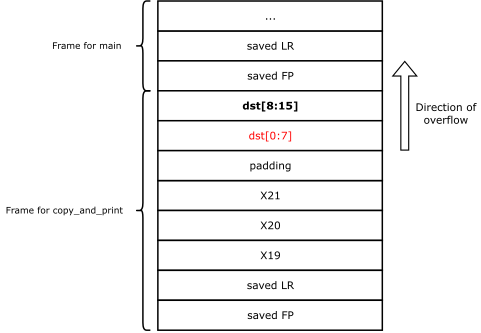
\includegraphics[width=0.8\textwidth,height=\textheight]{img/stack-buffer-overflow.pdf}
\caption{Stack frame layout for stack buffer overflow example}
\end{figure}

The exact details of the stack frame layout, including the ordering of
variables and the exact control information stored, will depend on the
specific compiler version you use and the architecture you compile for.

As can be seen the stack diagram, an overflowing write in function
\texttt{copy\_and\_print} can overwrite the saved frame pointer (FP) and
link register (LR) in \texttt{main}'s frame. When
\texttt{copy\_and\_print} returns, execution continues in \texttt{main}.
When \texttt{main} returns, however, execution continues from the
address stored in the saved LR, which has been overwritten. Therefore,
when an attacker can choose the value that overwrites the saved LR, it's
possible to control where the program resumes execution after returning
from \texttt{main}.

Before non-executable stacks were mainstream, a common way to exploit
these vulnerabilities would be to use the overflow to simultaneously
write shellcode\footnote{A shellcode is a short instruction sequence
  that performs an action such as starting a shell on the victim
  machine.}\index{shellcode} to the stack and overwrite the return
address so that it points to the shellcode.
(\protect\hyperlink{ref-AlephOne1996}{Aleph One 1996}) is a classic
example of this technique.

The obvious solution to this issue is to use memory protection features
of the processor in order to mark the stack (along with other data
sections) as non-executable\footnote{Note that the use of
  \href{https://gcc.gnu.org/onlinedocs/gcc/Nested-Functions.html}{nested
  functions} in GCC requires
  \href{https://gcc.gnu.org/onlinedocs/gccint/Trampolines.html}{trampolines}
  which reside on an executable stack. The use of nested functions,
  therefore, poses a security risk.}. However, even when the stack is
not executable, more advanced techniques can be used to exploit an
overflow that overwrites the return address. These take advantage of
code that already exists in the executable or in library code, and will
be described in the next section.

Stack canaries are an alternative mitigation for stack buffer overflows.
The general idea is to store a known value, called the stack canary,
between the buffer and the control information (in the example, the
saved FP and LR), and to check this value before leaving the function.
Since an overflow that would overwrite the return address is going to
overwrite the canary first, a corruption of the return address through a
stack buffer overflow will be detected.

This technique has a few limitations: first of all, it specifically aims
to protect against stack buffer overflows, and does nothing to protect
against stronger primitives (e.g.~arbitrary write primitives).
Control-flow integrity techniques, which are described in the next
section, aim to protect the integrity of stored code pointers against
any modification.

Secondly, since a compiler needs to generate additional instructions for
ensuring the canary's integrity, heuristics are usually employed to
determine which functions are considered vulnerable. The additional
instructions are then generated only for the functions that are
considered vulnerable. Since heuristics aren't always perfect, this
poses another potential limitation of the technique. To address this,
compilers can introduce various levels of heuristics, ranging from
applying the mitigations only to a small proportion of functions, to
applying it universally. See, for example, the
\texttt{-fstack-protector}, \texttt{-fstack-protector-strong} and
\texttt{-fstack-protector-all} options offered by both
\href{https://gcc.gnu.org/onlinedocs/gcc/Instrumentation-Options.html}{GCC}
and
\href{https://clang.llvm.org/docs/ClangCommandLineReference.html\#cmdoption-clang-fstack-protector}{Clang}.

Another limitation is the possibility of leaks of the canary value. The
canary value is often randomized at program start but remains the same
during the program's execution. An attacker who manages to obtain the
canary value at some point might, therefore, be able to reuse the leaked
canary value and corrupt control information while avoiding detection.
Choosing a canary value that includes a null byte (the C-style string
terminator) might help in limiting the damage of overflows coming from
string manipulation functions, even when the value is leaked.

Many buffer overflow vulnerabilities result from the use of unsafe
library functions, such as \texttt{gets}, or from the unsafe use of
library functions such as \texttt{strcpy}. There is extensive literature
on writing secure C/C++\index{C}\index{C++} code, for example
(\protect\hyperlink{ref-Seacord2013}{Seacord 2013}) and
(\protect\hyperlink{ref-Dowd2006}{Dowd, McDonald, and Schuh 2006}). A
different approach to limiting the effects of overflows is library
function hardening, which aims to detect buffer overflows and terminate
the program gracefully. This involves the introduction of feature macros
like \texttt{\_FORTIFY\_SOURCE}
(\protect\hyperlink{ref-Sharma2014}{Sharma 2014}).

Finally, it's important to mention that not all buffer overflows aim to
overwrite a saved return address. There are many cases where a buffer
overflow can overwrite other data adjacent to the buffer, for example an
adjacent variable that determines whether authorization was successful,
or a function pointer that, when modified, can modify the program's
control flow according to the attacker's wishes.

Some of these vulnerabilities can be mitigated with the measures
described in this section, but often more general measures to ensure
memory safety or \protect\hyperlink{cfi}{Control-Flow Integrity} are
necessary. For example, in addition to the hardening of specific library
functions, compilers can also implement automatic bounds checking for
arrays where the array bound can be statically determined
(\texttt{-fsanitize=bounds}), as well as various other ``sanitizers''.
We will describe these measures in following sections.

\hypertarget{code-reuse-attacks}{%
\section{Code reuse attacks}\label{code-reuse-attacks}}

In the early days of memory vulnerability exploitation, attackers could
simply place shellcode\index{shellcode} of their choice in executable
memory and jump to it. As non-executable stack and heap became
mainstream, attackers started to reuse code already present in an
application's binary and linked libraries instead. A variety of
different techniques to this effect came to light.

The simplest of these techniques is return-to-libc
(\protect\hyperlink{ref-Solar1997}{Solar Designer 1997}). Instead of
returning to shellcode that the attacker has injected, the return
address is modified to return into a library function, such as
\texttt{system} or \texttt{exec}. This technique is simpler to use when
arguments are also passed on the stack and can therefore be controlled
with the same stack buffer overflow that is used to modify the address.

\hypertarget{return-oriented-programming}{%
\subsection{Return-oriented
programming}\label{return-oriented-programming}}

Return-to-libc attacks restrict an attacker to whole library functions.
While this can lead to powerful attacks, it has also been demonstrated
that it is possible to achieve arbitrary computation by combining a
number of short instruction sequences ending in indirect control
transfer instructions, known as \textbf{gadgets}\index{gadget}. The
indirect control transfer instructions make it easy for an attacker to
execute gadgets one after another, by controlling the memory or register
that provides each control transfer instruction's target.

In return-oriented programming
(ROP)\index{return-oriented programming (ROP)}
(\protect\hyperlink{ref-Shacham2007}{Shacham 2007}), each gadget
performs a simple operation, for example setting a register, then pops a
return address from the stack and returns to it. The attacker constructs
a fake call stack (often called a ROP chain\index{ROP
chain}) which ensures a number of gadgets are executed one after
another, in order to perform a more complex operation.

This will hopefully become more clear with an example: a ROP chain for
AArch64 Linux that starts a shell, by calling \texttt{execve} with
\texttt{"/bin/sh"} as an argument.
\href{https://man7.org/linux/man-pages/man2/execve.2.html}{The prototype
of the \texttt{execve} library function}, which wraps the exec system
call, is:

\begin{verbatim}
  int execve(const char *pathname, char *const argv[],
             char *const envp[]);
\end{verbatim}

For AArch64, \texttt{pathname} will be passed in the \texttt{x0}
register, \texttt{argv} will be passed in \texttt{x1}, and \texttt{envp}
in \texttt{x2}. For starting a shell, it is sufficient to:

\begin{itemize}
\tightlist
\item
  Make \texttt{x0} contain a pointer to \texttt{"/bin/sh"}.
\item
  Make \texttt{x1} contain a pointer to an array of pointers with two
  elements:

  \begin{itemize}
  \tightlist
  \item
    The first element is a pointer to \texttt{"/bin/sh"}.
  \item
    The second element is zero (\texttt{NULL}).
  \end{itemize}
\item
  Make \texttt{x2} contain zero (\texttt{NULL}).
\end{itemize}

This can be achieved by chaining gadgets to set the registers
\texttt{x0}, \texttt{x1}, \texttt{x2}, and then returning to
\texttt{execve} in the C library.

Let's assume we have the following gadgets:

\begin{enumerate}
\def\labelenumi{\arabic{enumi}.}
\tightlist
\item
  A gadget that loads \texttt{x0} and \texttt{x1} from the stack:
\end{enumerate}

\begin{verbatim}
  gadget_x0_x1:
    ldp x0, x1, [sp]
    ldp x20, x19, [sp, #64]
    ldp x29, x30, [sp, #32]
    ldr x21, [sp, #48]
    add sp, sp, #0x50
    ret
\end{verbatim}

\begin{enumerate}
\def\labelenumi{\arabic{enumi}.}
\setcounter{enumi}{1}
\tightlist
\item
  A gadget that sets \texttt{x2} to zero, but also clears \texttt{x0} as
  a side-effect:
\end{enumerate}

\begin{verbatim}
  gadget_x2:
    mov x2, xzr
    mov x0, x2
    ldp x20, x19, [sp, #32]
    ldp x29, x30, [sp]
    ldr x21, [sp, #16]
    add sp, sp, #0x30
    ret
\end{verbatim}

\tododiv{Explain how these gadgets could result from C/C++ code. The
current versions are slightly tweaked by hand to have more manageable
offsets.
\href{https://github.com/llsoftsec/llsoftsecbook/issues/164}{\#164}}

Both gadgets also clobber several uninteresting registers, but since
\texttt{gadget\_x2} also clears \texttt{x0}, it becomes clear that we
should use a ROP chain that:

\begin{enumerate}
\def\labelenumi{\arabic{enumi}.}
\tightlist
\item
  Returns to \texttt{gadget\_x2}, which sets \texttt{x2} to zero.
\item
  Returns to \texttt{gadget\_x0\_x1}, which sets \texttt{x0} and
  \texttt{x1} to the desired values.
\item
  Returns to \texttt{execve}.
\end{enumerate}

Figure \protect\hyperlink{fig:rop-control-flow}{1} shows this control
flow.

\begin{figure}
\hypertarget{fig:rop-control-flow}{%
\centering
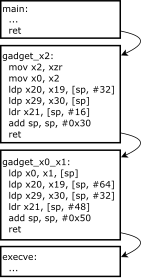
\includegraphics[width=0.3\textwidth,height=\textheight]{img/rop-control-flow.pdf}
\caption{Figure 1: ROP example control flow}\label{fig:rop-control-flow}
}
\end{figure}

\begin{figure}
\hypertarget{fig:rop-call-stack}{%
\centering
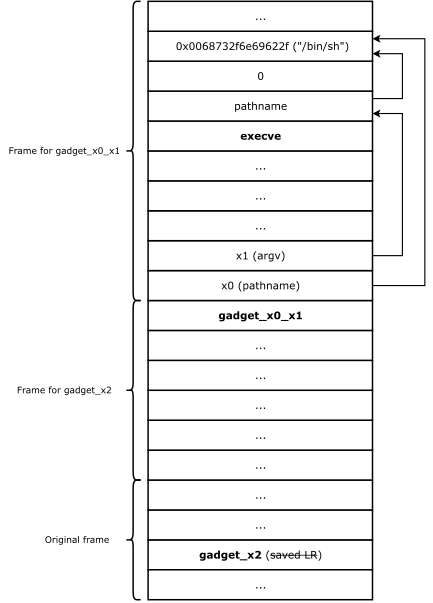
\includegraphics[width=0.8\textwidth,height=\textheight]{img/rop-call-stack.pdf}
\caption{Figure 2: ROP example fake call
stack}\label{fig:rop-call-stack}
}
\end{figure}

We can achieve this by constructing the fake call stack shown in figure
\protect\hyperlink{fig:rop-call-stack}{2}, where ``Original frame''
marks the frame in which the address of \texttt{gadget\_x2} has replaced
a saved return address that will be loaded and returned to in the
future. As an alternative, an attacker could place this fake call stack
somewhere else, for example on the heap, and use a primitive that
changes the stack pointer's value instead. This is known as stack
pivoting\index{stack pivoting}.

Note that this fake call stack contains NULL bytes, even without
considering the exact values of the various return addresses included.
An overflow bug that is based on a C-style string operation would not
allow an attacker to replace the stack contents with this fake call
stack in one go, since C-style strings are null-terminated and copying
the fake stack contents would stop once the first NULL byte is
encountered. The ROP chain would therefore need to be adjusted so that
it doesn't contain NULL bytes, for example by initially replacing the
NULL bytes with a different byte and adding some more gadgets to the ROP
chain that write zero to those stack locations.

A question that comes up when looking at the stack diagram is ``how do
we know the addresses of these gadgets''? We will talk a bit more about
this in the next section.

ROP gadgets like the ones used here may be easy to identify by visual
inspection of a disassembled binary, but it's common for attackers to
use ``gadget scanner''\index{gadget scanner} tools in order to discover
large numbers of gadgets automatically. Such tools can also be useful to
a compiler engineer working on a code reuse attack mitigation, as they
can point out code sequences that should be protected and have been
missed.

Anything in executable memory can potentially be used as a ROP gadget,
even if the compiler has not intended it to be code. This includes
literal pools which are intermingled with code, and, on architectures
with variable length instruction encoding, returning to the middle of an
instruction. In a JIT compiler where the attacker might influence what
literals are generated this can be particularly powerful. For example,
on x86, the compiler might have emitted the instruction
\texttt{mov\ \$0xc35f,\ \%ax} which is encoded as the four bytes
\texttt{66\ b8\ 5f\ c3}. If the attacker can divert execution two bytes
into that 4-byte instruction it will execute \texttt{5f\ c3}. Those
bytes corresponds to the two single byte instructions
\texttt{pop\ \%rdi;\ ret} which is a useful ROP gadget.

\hypertarget{jump-oriented-programming}{%
\subsection{Jump-oriented programming}\label{jump-oriented-programming}}

Jump-oriented programming (JOP)\index{jump-oriented programming (JOP)}
(\protect\hyperlink{ref-Bletsch2011}{Bletsch et al. 2011}) is a
variation on ROP, where gadgets can also end in indirect branch
instructions instead of return instructions. The attacker chains a
number of such gadgets through a dispatcher
gadget\index{dispatcher gadget}, which loads pointers one after another
from an array of pointers, and branches to each one in return. The
gadgets used must be set up so that they branch or return back to the
dispatcher after they're done. This is demonstrated in figure
\protect\hyperlink{fig:jop}{3}.

\begin{figure}
\hypertarget{fig:jop}{%
\centering
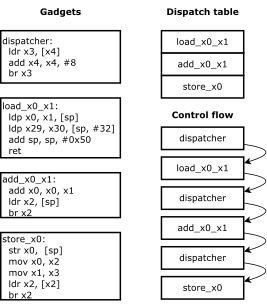
\includegraphics[width=0.5\textwidth,height=\textheight]{img/jop.pdf}
\caption{Figure 3: JOP example}\label{fig:jop}
}
\end{figure}

\tododiv{The gadgets in the figure are made up, chosen to highlight that
each gadget can end in a different type of indirect control flow
transfer instruction. Consider replacing them with more realistic ones.
\href{https://github.com/llsoftsec/llsoftsecbook/issues/165}{\#165}}

In figure \protect\hyperlink{fig:jop}{3}, \texttt{x4} initially points
to the ``dispatch table'', which has been modified by the attacker to
contain the addresses of the three gadgets they want to execute. The
dispatcher gadget loads each address in the dispatch table one by one
and branches to them. The first gadget loads \texttt{x0} and \texttt{x1}
from the stack, where the attacker has placed the inputs of their
choice. It then loads its return address, also modified by the attacker
so that it points back to the dispatcher gadget, and returns to it. The
dispatcher branches to the next gadget, which adds \texttt{x0} and
\texttt{x1} and leaves the result in \texttt{x0}, branching back to the
dispatcher through another value loaded from the stack into \texttt{x2}.
The final gadget stores the result of the addition, which remains in
\texttt{x0}, to the stack, before branching to \texttt{x2}, which still
points to the dispatcher gadget.

\hypertarget{counterfeit-object-oriented-programming}{%
\subsection{Counterfeit Object-oriented
programming}\label{counterfeit-object-oriented-programming}}

Counterfeit Object-oriented programming (COOP)\index{counterfeit
object-oriented programming (COOP)}
(\protect\hyperlink{ref-Schuster2015}{Schuster et al. 2015}) is a code
reuse technique that takes advantage of C++ \index{C++} virtual function
calls. A COOP attack takes advantage of existing virtual functions and
\href{https://en.wikipedia.org/wiki/Virtual_method_table}{vtables}, and
creates fake objects pointing to these existing vtables. The virtual
functions used as gadgets in the attack are called vfgadgets. To chain
vfgadgets together, the attacker uses a ``main loop gadget'', similar to
JOP's dispatcher gadget, which is itself a virtual function that loops
over a container of pointers to C++ objects and invokes a virtual
function on these objects.
(\protect\hyperlink{ref-Schuster2015}{Schuster et al. 2015}) describes
the attack in more detail. It is specifically mentioned here as an
example of an attack that doesn't depend on directly replacing return
addresses and code pointers, like ROP and JOP do. Such language-specific
attacks are important to consider when considering mitigations against
code reuse attacks, which will be the topic of the next section.

\hypertarget{sigreturn-oriented-programming}{%
\subsection{Sigreturn-oriented
programming}\label{sigreturn-oriented-programming}}

One last example of a code reuse attack that is worth mentioning here is
sigreturn-oriented programming
(SROP)\index{sigreturn-oriented programming
(SROP)} (\protect\hyperlink{ref-Bosman2014}{Bosman and Bos 2014}). It is
a special case of ROP where the attacker creates a fake signal handler
frame and calls \texttt{sigreturn}. \texttt{sigreturn} is a system call
on many UNIX-type systems which is normally called upon return from a
signal handler, and restores the state of the process based on the state
that has been saved on the signal handler's stack by the kernel
previously, on entry to the signal handler. The ability to fake a signal
handler frame and call \texttt{sigreturn} gives an attacker a simple way
to control the state of the program.

\hypertarget{mitigations-against-code-reuse-attacks}{%
\section{Mitigations against code reuse
attacks}\label{mitigations-against-code-reuse-attacks}}

When discussing mitigations against code reuse attacks, it is important
to keep in mind that there are two capabilities the attacker must have
for such attacks to work:

\begin{itemize}
\tightlist
\item
  the ability to overwrite return addresses or function pointers
\item
  knowledge of the target addresses to overwrite them with (e.g.~libc
  function entry points).
\end{itemize}

When code reuse attacks were first described, programs used to contain
absolute code pointers, and needed to be loaded at fixed addresses. The
stack base was predictable, and libraries were loaded in predictable
memory locations. This made code reuse attacks simple, as all of the
addresses needed for a successful exploit were easy to discover.

\hypertarget{aslr}{%
\subsection{ASLR}\label{aslr}}

\href{https://en.wikipedia.org/wiki/Address_space_layout_randomization}{Address
space layout randomization (ASLR)}\index{ASLR} makes this more difficult
by randomizing the positions of the memory areas containing the
executable, the loaded libraries, the stack and the heap. ASLR requires
code to be position-independent. Given enough entropy, the chance that
an attacker would successfully guess one or more addresses in order to
mount a successful attack will be greatly reduced.

Does this mean that code reuse attacks have been made redundant by ASLR?
Unfortunately, this is not the case. There are various ways in which an
attacker can discover the memory layout of the victim program. This is
often referred to as an ``info leak''\index{info leak}
(\protect\hyperlink{ref-Serna2012}{Serna 2012}).

Since we can not exclude code reuse attacks solely by making addresses
hard to guess, we need to also consider mitigations that prevent
attackers from overwriting return addresses and other code pointers.
Some of the mitigations described
\protect\hyperlink{stack-buffer-overflows}{earlier}, like stack canaries
and library function hardening, can help in specific situations, but for
the more general case where an attacker has obtained arbitrary read and
write primitives, we need something more.

\hypertarget{cfi}{%
\subsection{CFI}\label{cfi}}

\href{https://en.wikipedia.org/wiki/Control-flow_integrity}{Control-flow
integrity (CFI)}\index{CFI} is a family of mitigations that aim to
preserve the intended control flow of a program. This is done by
restricting the possible targets of indirect branches and returns. A
scheme that protects indirect jumps and calls is referred to as
forward-edge CFI\index{forward-edge CFI}, whereas a scheme that protects
returns is said to implement backward-edge CFI\index{backward-edge CFI}.
Ideally, a CFI scheme would not allow any control flow transfers that
don't occur in a correct program execution, however different schemes
have varying granularities. They often rely on function type checks or
use static analysis (points-to analysis) to identify potential control
flow transfer targets. (\protect\hyperlink{ref-Burow2017}{Burow et al.
2017}) compares a number of available CFI schemes based on the
precision. For forward-edge CFI schemes, for example, schemes are
classified based on whether or not they perform, among others,
flow-sensitive analysis, context-sensitive analysis and class-hierarchy
analysis.

\hypertarget{clang-cfi}{%
\subsubsection{Clang CFI}\label{clang-cfi}}

\href{https://clang.llvm.org/docs/ControlFlowIntegrity.html}{Clang's
CFI} includes a variety of forward-edge control-flow integrity checks.
These include checking that the target of an indirect function call is
an address-taken function of the correct type and checking that a C++
\index{C++} virtual call happens on an object of the correct dynamic
type.

For example, assume we have a class \texttt{A} with a virtual function
\texttt{foo} and a class \texttt{B} deriving from \texttt{A}, and that
these classes are not exported to other compilation modules:

\begin{verbatim}
class A {
public:
  virtual void foo() {}
};

class B : public A {
public:
  virtual void foo() {}
};

void call_foo(A* a) {
  a->foo();
}
\end{verbatim}

When compiling with \texttt{-fsanitize=cfi\ -flto\ -fvisibility=hidden}
\footnote{The LTO and visibility flags are required by Clang's CFI.},
the code for \texttt{call\_foo} would look something like this:

\begin{verbatim}
00000000004006b4 <call_foo(A*)>:
  4006b4:       a9bf7bfd        stp     x29, x30, [sp, #-16]!
  4006b8:       910003fd        mov     x29, sp
  4006bc:       f9400008        ldr     x8, [x0]
  4006c0:       90000009        adrp    x9, 400000 <_init-0x558>
  4006c4:       91216129        add     x9, x9, #0x858
  4006c8:       cb090109        sub     x9, x8, x9
  4006cc:       d1004129        sub     x9, x9, #0x10
  4006d0:       93c91529        ror     x9, x9, #5
  4006d4:       f100093f        cmp     x9, #0x2
  4006d8:       540000a2        b.cs    4006ec <call_foo(A*)+0x38>
  4006dc:       f9400108        ldr     x8, [x8]
  4006e0:       d63f0100        blr     x8
  4006e4:       a8c17bfd        ldp     x29, x30, [sp], #16
  4006e8:       d65f03c0        ret
  4006ec:       d4200020        brk     #0x1
\end{verbatim}

This code looks complicated, but what it does is check that the virtual
table pointer (vptr) of the argument points to the vtable of \texttt{A}
or of \texttt{B}, which are stored consecutively and are the only
allowed possibilities. The checks generated for different types of
control-flow transfers are similar.

Another implementation of forward-edge CFI is Windows
\href{https://docs.microsoft.com/en-us/windows/win32/secbp/control-flow-guard}{Control
Flow Guard}, which only allows indirect calls to functions that are
marked as valid indirect control flow targets.

\hypertarget{clang-shadow-stack}{%
\subsubsection{Clang Shadow Stack}\label{clang-shadow-stack}}

Clang also implements a backward-edge CFI scheme known as
\href{https://clang.llvm.org/docs/ShadowCallStack.html}{Shadow
Stack}\index{shadow stack}. In Clang's implementation, a separate stack
is used for return addresses, which means that stack-based buffer
overflows cannot be used to overwrite return addresses. The address of
the shadow stack is randomized and kept in a dedicated register, with
care taken so that it is never leaked, which means that an arbitrary
write primitive cannot be used against the shadow stack unless its
location is discovered through some other means.

As an example, when compiling with
\texttt{-fsanitize=shadow-call-stack\ -ffixed-x18} \footnote{The
  \texttt{-ffixed-x18} flag results in treating the \texttt{x18}
  register as reserved, and is required by
  \texttt{-fsanitize=shadow-call-stack} on some platforms.}, the code
generated for the \texttt{main} function from the
\protect\hyperlink{stack-buffer-overflow}{earlier stack buffer overflow
example} will look something like:

\begin{verbatim}
main:
    cmp w0, #2
    b.lt    .LBB1_2
    str x30, [x18], #8
    stp x29, x30, [sp, #-16]!
    mov x29, sp
    ldr x0, [x1, #8]
    bl  copy_and_print
    ldp x29, x30, [sp], #16
    ldr x30, [x18, #-8]!
.LBB1_2:
    mov w0, wzr
    ret
\end{verbatim}

You can see that the shadow stack address is kept in \texttt{x18}. The
return address is also saved on the ``normal'' stack for compatibility
with unwinders, but it's not actually used for the function return.

\hypertarget{pointer-authentication}{%
\subsubsection{Pointer Authentication}\label{pointer-authentication}}

In addition to software implementations, there are a number of
hardware-based CFI implementations. A hardware-based implementation has
the potential to offer improved protection and performance compared to
an equivalent software-only CFI scheme.

One such example is Pointer Authentication\index{Pointer Authentication}
(\protect\hyperlink{ref-Rutland2017}{Rutland 2017}), an Armv8.3 feature,
supported only in AArch64 state, that can be used to mitigate code reuse
attacks. Pointer Authentication introduces instructions that generate a
pointer \emph{signature}, called a Pointer Authentication Code (PAC),
based on a key and a modifier. It also introduces matching instructions
to authenticate this signature. Incorrect authentication leads to an
unusable pointer, that will cause a fault when used \footnote{With the
  FPAC extension, a fault is raised at incorrect authentication.}. The
key is not directly accessible by user space software.

Pointers are stored as 64-bit values, but they don't need all of these
bits to describe the available address space, so a number of bits in the
top of each pointer are unused. The unused bits must be all ones or all
zeros, so we refer to them as extension
bits\index{pointer extension bits}. Pointer Authentication Codes are
stored in those unused extension bits of a pointer. The exact number of
PAC bits depends on the number of unused pointer bits, which varies
based on the configuration of the virtual address space size.\footnote{If
  the Top-Byte-Ignore (TBI)\index{Top-Byte-Ignore (TBI)} feature is
  enabled, the top byte of pointers is ignored when performing memory
  accesses. This restricts the number of available PAC bits.}

\href{https://clang.llvm.org/docs/ClangCommandLineReference.html\#aarch64}{Clang}
and \href{https://gcc.gnu.org/onlinedocs/gcc/AArch64-Options.html}{GCC}
both use Pointer Authentication for return address signing, when
compiling with the \texttt{-mbranch-protection=pac-ret} flag. When
compiling with Clang using this flag, the \texttt{main} function from
the \protect\hyperlink{stack-buffer-overflow}{earlier stack buffer
overflow example} looks like:

\begin{verbatim}
main:
    cmp w0, #2
    b.lt    .LBB1_2
    paciasp
    stp x29, x30, [sp, #-16]!
    ldr x0, [x1, #8]
    mov x29, sp
    bl  copy_and_print
    ldp x29, x30, [sp], #16
    autiasp
.LBB1_2:
    mov w0, wzr
    ret
\end{verbatim}

Notice the \texttt{paciasp} and \texttt{autiasp} instructions:
\texttt{paciasp} computes a PAC for the return address in the link
register (\texttt{x30}), based on the current value of the stack pointer
(\texttt{sp}) and a key. This PAC is inserted in the extension bits of
the pointer. We then store this signed version of the link register on
the stack. Before returning, we load the signed return address from the
stack, we execute \texttt{autiasp}, which verifies the PAC stored in the
return address, again based on the value of the key and the value of the
stack pointer (which at this point will be the same as when we signed
the return address). If the PAC is correct, which will be the case in
normal execution, the extension bits of the address are restored, so
that the address can be used in the \texttt{ret} instruction. However,
if the stored return address has been overwritten with an address with
an incorrect PAC, the upper bits will be corrupted so that subsequent
uses of the address (such as in the \texttt{ret} instruction) will
result in a fault.

By making sure we don't store any return addresses without a PAC, we can
significantly reduce the effectiveness of ROP attacks: since the secret
key is not retrievable by an attacker, an attacker cannot calculate the
correct PAC for a given address and modifier, and is restricted to
guessing it. The probability of success when guessing a PAC depends on
the exact number of PAC bits available in a given system configuration.
However, authenticated pointers are vulnerable to pointer substitution
attacks\index{pointer substitution
attack}, where a pointer that has been signed with a given modifier is
replaced with a different pointer that has also been signed with the
same modifier.

Another backward-edge CFI scheme that uses Pointer Authentication
instructions is PACStack
(\protect\hyperlink{ref-Liljestrand2021}{Liljestrand et al. 2021}),
which chains together PACs in order to include the full context (all of
the previous return addresses in the call stack) when signing a return
address. \todospan{{Add more references to relevant research
\href{https://github.com/llsoftsec/llsoftsecbook/issues/166}{\#166}}}

Pointer Authentication can also be used more widely, for example to
implement a forward-edge CFI scheme, as is done in the arm64e ABI
(\protect\hyperlink{ref-McCall2019}{McCall and Bougacha 2019}). The
Pointer Authentication instructions, however, are generic enough to also
be useful in implementing more general memory safety measures, beyond
CFI. \todospan{{Mention more Pointer Authentication uses in later
section, and add link here
\href{https://github.com/llsoftsec/llsoftsecbook/issues/167}{\#167}}}

\hypertarget{bti}{%
\subsubsection{BTI}\label{bti}}

\href{https://developer.arm.com/documentation/102433/0100/Jump-oriented-programming?lang=en}{Branch
Target Identification (BTI)} \index{BTI}, introduced in Armv8.5, offers
coarse-grained forward-edge protection. With BTI, the locations that are
targets of indirect branches have to be marked with a new instruction,
\texttt{BTI}. There are four different types of BTI instructions that
permit different types of indirect branches (indirect jump, indirect
call, both, or none). An indirect branch to a non-BTI instruction or the
wrong type of BTI instruction will raise a Branch Target Exception.

Both Clang and GCC support generating BTI instructions, with the
\texttt{-mbranch-protection=bti} flag, or, to enable both BTI and return
address signing with Pointer Authentication,
\texttt{-mbranch-protection=standard}.

Two aspects of BTI can simplify its deployment: individual pages can be
marked as guarded or unguarded, with BTI checks as described above only
applying to indirect branches targeting guarded pages. In addition to
this, the BTI instruction has been assigned to the hint space, therefore
it will be executed as a no-op in cores that do not support BTI, aiding
its adoption.

\hypertarget{cfi-implementation-pitfalls}{%
\subsubsection{CFI implementation
pitfalls}\label{cfi-implementation-pitfalls}}

When implementing CFI measures like the ones described here, it is
important to be aware of known weaknesses that affect similar schemes.
(\protect\hyperlink{ref-Conti2015}{Conti et al. 2015}) describes how CFI
implementations can suffer when certain registers are spilled on the
stack, where they could be controlled by an attacker. For example, if a
register that contains a function pointer that has just been validated
gets spilled, the check can effectively be bypassed by overwriting the
spilled pointer.

Having discussed various mitigations against code reuse attacks, it's
time to turn our attention to a different type of attacks, which do not
try to overwrite code pointers: attacks against non-control data, which
will be the topic of the next section.

\hypertarget{non-control-data-attacks}{%
\section{Non-control data attacks}\label{non-control-data-attacks}}

In the previous sections, we have focused on subverting control flow by
overwriting control data\index{control data}, which are used to change
the value of the program counter, such as return addresses and function
pointers. Since these types of attacks are prominent, many mitigations
have been designed with the goal of maintaining control-flow integrity.
Non-control data attacks\index{non-control data attacks}, also known as
data-only attacks\index{data-only attacks}, can completely bypass these
mitigations, since the data they modify is not the control data that
these mitigations protect.

Non-control data attacks can range from very simple attacks targeting a
single piece of data to very elaborate attacks with very high
expressiveness (\protect\hyperlink{ref-Beer2021}{Beer and Groß 2021}). A
very simple example may look something like this:

\begin{verbatim}
// Returns zero for failure, non-zero for success.
int authenticate() {
  int authenticated = 0;
  char passphrase[10];
  if (fgets(passphrase, 20, stdin)) {     // buffer overflow
    if (!strcmp(passphrase, "secret\n")) {
      authenticated = 1;
    }
  }
  return authenticated;
}
\end{verbatim}

The example shows a simplified\footnote{This is obviously not a
  realistic example of how authentication should be done, but simply
  serves to illustrate how a buffer overflow into a non-control variable
  can have serious security consequences.} function that reads a
passphrase from a user, compares it with a known value and sets an
integer stack variable to indicate whether ``authentication'' was
successful or not. The function contains a very obvious buffer overflow,
as the string length limit passed to \texttt{fgets} does not match the
buffer size.

Figure \protect\hyperlink{fig:non-control-data-attack}{4} shows the
stack frame layout for this function when the code is compiled for
AArch64 with Clang 10.0\footnote{The stack frame layout may be
  significantly different for other architectures and compilers.}. As
the figure shows, an overflow of \texttt{passphrase} will overwrite
\texttt{authenticated}, setting it to a non-zero value, even though the
passphrase was incorrect. The \texttt{authenticate} function will then
return a non-zero value, incorrectly indicating authentication success.

\begin{figure}
\hypertarget{fig:non-control-data-attack}{%
\centering
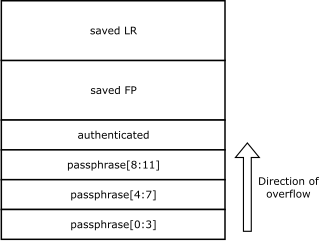
\includegraphics[width=0.6\textwidth,height=\textheight]{img/non-control-data-attack.pdf}
\caption{Figure 4: Stack frame for
\texttt{authenticate}}\label{fig:non-control-data-attack}
}
\end{figure}

For many more simple examples of data-only attacks that can occur in
real applications, see (\protect\hyperlink{ref-Chen2005}{Chen et al.
2005}). Although this makes it clear that data-only attacks are a real
issue, it leaves open a very important question: what are the limits of
such attacks? It is tempting to assume that data-only attacks are
somehow inherently limited, however it has been demonstrated in
(\protect\hyperlink{ref-Hu2016}{Hu et al. 2016}) that they can, in fact,
be very expressive. (\protect\hyperlink{ref-Hu2016}{Hu et al. 2016})
describes Data-Oriented Programming (DOP), a general method for building
data-only attacks against a vulnerable program, starting from a known
memory error in the program\footnote{The authors describe how DOP
  gadgets can be chained to simulate a Turing machine, making DOP
  attacks Turing-complete (it's not possible to simulate the infinite
  tape of a Turing machine on any actual hardware, of course).
  Turing-completeness is not, however, a particularly useful measure of
  exploitability, as explained in
  (\protect\hyperlink{ref-Dullien2018}{Flake 2018}). Many applications
  offer their users the ability to perform arbitrary computation, for
  example JavaScript engines, and those capabilities can be useful to an
  attacker, but performing a computation without affecting normal
  program behavior does not constitute ``exploitation''.}.

The authors of (\protect\hyperlink{ref-Hu2016}{Hu et al. 2016}) describe
a small language called MINDOP, with a virtual instruction set and
virtual registers. The virtual registers of MINDOP correspond to memory
locations. The MINDOP instructions correspond to operations on these
virtual registers, for example loading a value into a virtual register,
storing a value from a virtual register, arithmetic operations and even
conditional and unconditional jumps. The authors show how to identify
gadgets in the code that implement the various MINDOP instructions and
are reachable from memory errors, and how those gadgets can be stitched
together with the help of dispatcher gadgets, the role of which is
specifically to chain gadgets together.

Stitching gadgets together is simpler for interactive attacks, where the
attacker can keep providing malicious input to trigger the initial
memory error and a certain chain of gadgets, as many times as needed.
For non-interactive attacks, the MINDOP jump operations are required as
well, used in conjunction with a memory location that provides a virtual
program counter.

The process of creating a DOP attack is not so simple and not fully
automated. Related literature
(\protect\hyperlink{ref-Ispoglou2018}{Ispoglou et al. 2018}) focuses on
automating data-only attacks.

When reading write-ups on recent security issues, instead of terminology
related to data-oriented gadgets, you are more likely to encounter the
term ``primitive'', which has been described in
\protect\hyperlink{exploitation-primitives}{an earlier section}. These
concepts are related: an arbitrary read primitive, for example, can be
produced by chaining a (possibly large) number of DOP gadgets. Talking
about primitives offers a nicer level of abstraction, as it tends to be
simpler to reason in terms of higher-level operations instead of many
small pieces of code that need to be stitched together to perform the
operations.

To summarize, data-only attacks are a significant concern. As most of
the mitigation techniques we have seen so far are control-flow oriented,
they are by design inadequate to protect against this different type of
attacks. In the next section, we will look at what we can do to address
them at their source: memory errors.

\hypertarget{preventing-and-detecting-memory-errors}{%
\section{Preventing and detecting memory
errors}\label{preventing-and-detecting-memory-errors}}

We have so far discussed how languages that are
\protect\hyperlink{a-bit-of-background-on-memory-vulnerabilities}{not
memory safe}, like C and C++, are vulnerable to memory errors and
therefore exploitation. In this section, we will discuss tools that are
available to C/C++ \index{C}\index{C++}programmers to help them detect
vulnerabilities that can lead to memory errors.

\hypertarget{sanitizers}{%
\subsection{Sanitizers}\label{sanitizers}}

Sanitizers \index{sanitizers} are tools that detect bugs during program
execution. Sanitizers usually have two components: a compiler
instrumentation part that introduces the new checks, and a runtime
library part. They are often too expensive to run in production mode, as
they tend to increase execution time and memory usage. They are commonly
used during testing of an application, frequently in combination with
fuzzers\index{fuzzing}\footnote{\href{https://en.wikipedia.org/wiki/Fuzzing}{Fuzzing}
  \index{fuzzing} is a powerful testing technique that relies on
  automatically generating large amounts of random inputs to the program
  under test.}.

A very popular sanitizer is
\href{https://clang.llvm.org/docs/AddressSanitizer.html}{Address
Sanitizer} (ASan)\index{AddressSanitizer (ASan)}. It aims to detect
various memory errors. These include out-of-bounds accesses,
use-after-free, double-free and invalid free\footnote{ASan also includes
  a \href{https://clang.llvm.org/docs/LeakSanitizer.html}{memory leak
  detector} \index{LeakSanitizer}.}. There are Address Sanitizer
implementations for both GCC \index{GCC} and Clang\index{Clang}, but we
will focus on the Clang implementation here.

ASan uses shadow memory\index{shadow memory} to keep track of the state
of the application's memory. Each byte of shadow memory records
information on 8 bytes of the application's memory. It represents how
many of the 8 bytes are addressable. When none of the bytes are
addressable, it encodes additional details (whether the 8 bytes are
out-of-bounds stack, out-of-bounds heap, freed memory, and so on).
Requiring one byte of shadow memory for every 8 bytes of application
memory means that ASan needs to reserve one-eighth of the application's
virtual address space (\protect\hyperlink{ref-Serebryany2012}{Serebryany
et al. 2012}). Shadow memory is allocated in one contiguous chunk, which
keeps mapping application memory to shadow memory simple.

ASan's runtime library replaces memory allocation functions like
\texttt{malloc}\index{malloc} and \texttt{free}\index{free} with its own
specialized versions. \texttt{malloc} introduces redzones\index{redzone}
before and after each allocation, which are marked as unaddressable.
\texttt{free} marks the entire allocation as unaddressable and places it
in quarantine, so that it doesn't get reallocated for a while (in a FIFO
basis). This allows for detecting use-after-free. The runtime library
also handles management of the shadow memory.

ASan's code instrumentation in the compiler introduces redzones around
each stack array allocation, and around globals. It then instruments
loads and stores to check whether the accessed memory is addressable,
based on the information stored in the shadow memory, and reports an
error if unaddressable memory is accessed.

ASan doesn't produce false positives and is easy to use. It requires
compiling and linking a program with the \texttt{-fsanitize=address}
option. It is used in practice for testing
\href{https://chromium.googlesource.com/chromium/src/+/HEAD/docs/asan.md}{large
projects}. There is a similar tool for dynamic memory error detection in
the Linux kernel,
\href{https://www.kernel.org/doc/html/v5.0/dev-tools/kasan.html}{KASAN}\index{KASAN}.

ASan's biggest drawback is its high runtime overhead and memory usage,
due to the quarantine, redzones and shadow memory.
\href{https://clang.llvm.org/docs/HardwareAssistedAddressSanitizerDesign.html}{Hardware-assisted
AddressSanitizer (HWASAN)} \index{HWASAN} works similarly to ASan, but
with partial hardware assistance can result in lower memory overheads,
at the cost of being less portable.

On AArch64\index{AArch64}, HWASAN uses Top-Byte Ignore
(TBI)\index{Top-Byte
Ignore (TBI)}. When TBI is enabled, the top byte of a pointer is ignored
when performing a memory access, allowing software to use that top byte
to store metadata, without affecting execution. Each allocation is
aligned to 16 bytes and each 16-byte chunk of memory (called
``granule'') is randomly assigned an 8-bit tag. The tag is stored in
shadow memory and is also placed in the top byte of the pointer to the
object. Memory loads and stores are then instrumented to check that the
tag stored in the pointer matches the tag stored in memory, and report
an error when a mismatch happens. \todospan{{Add diagram to demonstrate
how HWASAN works
\href{https://github.com/llsoftsec/llsoftsecbook/issues/168}{\#168}}}

For granules shorter than 16 bytes, the value stored in shadow memory is
not the actual tag, but the length of the granule. The actual tag is
stored at the last byte of the granule itself. For tags in shadow memory
with values between 1 and 15, HWASAN checks that the access is within
the bounds of the granule and the pointer tag matches the tag stored at
the last byte of the granule.

HWASAN is also easy to use, and simply requires compiling and linking an
application with the \texttt{-fsanitize=hwaddress} flag.

\href{https://llvm.org/docs/MemTagSanitizer.html}{MemTagSanitizer}\index{MemTagSanitizer}
goes one step further and uses the Armv8.5-A
\href{https://developer.arm.com/documentation/102925/0100}{Memory
Tagging Extension (MTE)}\index{Memory
Tagging Extension (MTE)}. With MTE, the tag checking is done
automatically by hardware, and an exception is raised on mismatch. MTE's
granule size is 16 bits, whereas tags are 4-bit. \todospan{{Consider
adding a whole section on MTE and its applications
\href{https://github.com/llsoftsec/llsoftsecbook/issues/169}{\#169}}}

\href{https://clang.llvm.org/docs/UndefinedBehaviorSanitizer.html\#ubsan-checks}{UndefinedBehaviorSanitizer
(UBSan)} \index{UBSan}detects undefined behavior during program
execution, for example array out-of-bounds accesses for statically
determined array bounds, null pointer dereference, signed integer
overflow and various kinds of integer conversions that result in data
loss. Although some of these checks are not directly related to memory
errors, these kinds of errors can lead to incorrect pointer arithmetic,
incorrect allocation sizes, and other issues that lead to memory errors,
so it is important to detect them and address them.

UBSan's documentation describes the full list of available checks. The
majority of these checks are enabled with the
\texttt{-fsanitize=undefined} flag, but there are also other useful
groupings of checks, for example \texttt{-fsanitize=integer} for checks
related to integer conversions and arithmetic.

There are many other sanitizers, more than can reasonably be covered in
this section. For the interested reader, we list a few more:

\begin{itemize}
\tightlist
\item
  \href{https://clang.llvm.org/docs/MemorySanitizer.html}{MemorySanitizer}\index{MemorySanitizer}:
  detects uninitialized reads.
\item
  \href{https://clang.llvm.org/docs/ThreadSanitizer.html}{ThreadSanitizer}\index{ThreadSanitizer}:
  detects data races.
\item
  \href{https://llvm.org/docs/GwpAsan.html}{GWP-ASan}\index{GWP-ASan}:
  detects use-after-free and heap buffer overflows, with low overhead
  that makes it suitable for production environments. It performs checks
  only on a sample of allocations.
\end{itemize}

\tododiv{Describe other mechanisms for detecting memory errors, both
software-based (static analysis, library and buffer hardening) and
hardware-based, e.g.~PAuth-based pointer integrity schemes, MTE etc
\href{https://github.com/llsoftsec/llsoftsecbook/issues/170}{\#170}}

\hypertarget{bounds-checking}{%
\subsection{Bounds checking}\label{bounds-checking}}

Making sure that memory accesses happen within the bounds of each
object's allocation is a very important part of memory safety. This is
usually described with the term ``spatial memory
safety''\index{spatial memory safety}. Out-of-bounds accesses result in
restricted read/write primitives\index{read
primitive}\index{write primitive}\footnote{These primitives are
  restricted since they can only access a limited number of bytes past
  the end of the allocation.}. An attacker can often easily convert
these into arbitrary read/write primitives. For example, this can be
achieved by overwriting pointer fields in allocations following the
object that was the target of the problematic memory access.

The C and C++ memory languages do not, as a general rule, perform bounds
checking\footnote{Some C++ containers have accessors that do perform
  bounds checking, for example \texttt{std::array::at()} and
  \texttt{std::vector::at()}.}. This is one of the sources of memory
errors in C/C++ programs. However, compilers have a history of
introducing bounds checks, even though the language does not require
them, in an effort to improve security of existing C/C++ codebases.

One of the simplest compiler options is \texttt{-Warray-bounds}, which
warns when an array access is always out of bounds. This is therefore
restricted to arrays with statically known size. This option is
supported by both GCC and Clang.

Another option supported by both compilers is
\texttt{-fsanitize=bounds}, included in
\protect\hyperlink{sanitizers}{UBSan}, which checks the bounds for
accesses to statically sized arrays at runtime. This handles more cases
than \texttt{-Warray-bounds}, as it can also check accesses to dynamic
indices. However, it's still limited, as it cannot perform bounds checks
on dynamically sized arrays, and it is still restricted to array bounds
checking. A more comprehensive solution would also cover pointers in
general, especially if pointer arithmetic is performed.

You may notice that there is a bit of overlap between the bounds checks
introduced by \texttt{-fsanitize=bounds} and the Address Sanitizer.
Although the scope of \texttt{-fsanitize=bounds} is restricted to
statically sized arrays, it's interesting to note that it can still
catch intra-object overflows\index{intra-object overflow} on array
member accesses that the Address Sanitizer would not, because the access
is still technically within the allocation. For example, given the
following code:

\begin{verbatim}
struct foo {
  int a[6];
  int b;
};

int get(struct foo *x, int i) {
  return x->a[i];
}
\end{verbatim}

a call to \texttt{get(f,\ 6)} will give an error with
\texttt{-fsanitize=bounds}, but not with \texttt{-fsanitize=address}.

Clang and GCC also support two builtin functions that return information
on the size of a variable. \texttt{\_\_builtin\_object\_size} can be
used for objects of statically known size and always evaluates at
compile time, whereas \texttt{\_\_builtin\_dynamic\_object\_size} can
also propagate dynamic information from allocation functions that have
been marked with the
\href{https://gcc.gnu.org/onlinedocs/gcc-4.7.2/gcc/Function-Attributes.html}{\texttt{alloc\_size}
function attribute}. These two builtins can be then used to introduce
bounds checks in user or library code. For example, the
\href{https://man7.org/linux/man-pages/man7/feature_test_macros.7.html}{\texttt{\_FORTIFY\_SOURCE}
macro} instructs \texttt{glibc} to introduce bounds checks in various
string and memory manipulation functions, such as \texttt{memcpy}. The
number of checks increases as the value of the macro increases (the used
values are currently 1-3). For example, the lower two levels won't use
the \texttt{\_\_builtin\_dynamic\_object\_size} builtin, as it has a
runtime overhead, additional to that of the checks themselves.

In order to support bounds checking for dynamically sized arrays, a
recent proposal for
\href{https://gcc.gnu.org/bugzilla/show_bug.cgi?id=108896}{GCC} and
\href{https://reviews.llvm.org/D148381}{Clang} proposes the addition of
a struct member attribute, \texttt{element\_count}. This attribute will
apply to
\href{https://en.wikipedia.org/wiki/Flexible_array_member}{flexible
array members} in structs, indicating another member of the struct that
expresses the array's length.

The
\href{https://discourse.llvm.org/t/rfc-enforcing-bounds-safety-in-c-fbounds-safety/70854}{\texttt{-fbounds-safety}}
proposal goes a bit further, introducing a similar annotation that can
be applied to pointers more generally. The proposal also aims to reduce
the annotation burden placed on programmers by only requiring the
annotations at
\href{https://en.wikipedia.org/wiki/Application_binary_interface}{ABI}\index{Application
binary interface (ABI)} boundaries\footnote{This refers to the interface
  between different binary modules, typically a user program and a
  system library. The ABI describes low-level details of that interface,
  for example the assignment of arguments and return values into
  registers or memory. In many systems, the ABI is expected to change
  rarely, so programs and libraries can be updated independently and
  still work together. This makes ABI changes undesirable, which is why
  this proposal aims to minimise them.}. Local variables which do not
cross ABI boundaries are implicitly converted to use wide pointers.
These wide pointers store bounds information alongside the original
pointer.

There are also hardening efforts focusing on C++ codebases. For example,
the \href{https://libcxx.llvm.org/Hardening.html}{libc++ hardening
modes} enable a number of assertions that aim to catch undefined
behaviour in the library. The
\href{https://discourse.llvm.org/t/rfc-c-buffer-hardening/65734}{C++
Buffer Hardening proposal} aims to extend this library hardening. The
proposal will also introduce a programming model in which all pointer
arithmetic is considered unsafe. Pointer arithmetic will have to be
replaced with alternatives from the C++ library, for example
\texttt{std::array}. The implementation of these alternatives in the
hardened library will include bounds checks.

Successfully using bounds checking compiler features for a large
codebase requires substantial effort. An example of this is refactoring
the Linux kernel to use bounds checks for flexible arrays, as described
in (\protect\hyperlink{ref-Cook2023}{Cook 2023}).

There are also hardware-based mitigations for violations of spatial
memory safety. For example,
\href{https://www.cl.cam.ac.uk/research/security/ctsrd/cheri/}{CHERI}
introduces \emph{capabilities}\index{capability} to conventional
Instruction Set Architectures. Capabilities combine a virtual address
with metadata that describes its corresponding bounds and permissions.
Capabilities cannot be forged, and can thus provide very strong
guarantees. Arm has developed a prototype architecture that adapts
CHERI, as well as a prototype SoC and development board, as part of the
\href{https://www.arm.com/architecture/cpu/morello}{Arm Morello
Program}.

Of course, another approach to mitigating spatial memory safety
vulnerabilities is using a language that has been designed with spatial
memory safety in mind. Such languages make sure that all memory accesses
are checked, either at compile-time or runtime. For example, the
\href{https://www.rust-lang.org/}{Rust programming language} introduces
bounds checks whenever the compiler cannot prove that an access is
within bounds\footnote{Rust also provides features that provide temporal
  memory safety and thread safety.}. There are many other memory safe
languages, with different characteristics. One example is JavaScript, a
dynamically typed, usually
\protect\hyperlink{jit-compiler-vulnerabilities}{JIT-compiled} language.
We'll discuss some of the issues that arise when implementing support
for such a language in the next section.

\hypertarget{jit-compiler-vulnerabilities}{%
\section{JIT compiler
vulnerabilities}\label{jit-compiler-vulnerabilities}}

Compiler correctness is obviously very important, as miscompilation
creates buggy programs even when the source code has no bugs. What might
be less obvious is that these bugs can have security implications. For
example, they can introduce memory safety errors in languages that are
otherwise memory safe. In some cases, a bug might leave most programs
unaffected and not cause security issues in practice before it is
detected and fixed. This is, of course, assuming that the bug has not
been \protect\hyperlink{supply-chain-attacks}{intentionally injected in
the compiler}.

Compiler bugs are an interesting source of security issues for
\href{https://en.wikipedia.org/wiki/Just-in-time_compilation}{just-in-time
(JIT)} compilers\index{JIT compilers}\footnote{JIT compilers compile
  code during execution of a program, as opposed to the more traditional
  compilation where code is compiled before the program is executed.}.
JIT compilation is often used in programs that receive source code as
input during program execution, for example in web browsers, for
executing JavaScript code included in web pages. In this context, the
input to the JIT compiler comes from arbitrary websites and is therefore
untrusted. Bugs in such JIT compilers can lead to compromise of the
whole program (here, the browser) if a malicious input (e.g.~coming from
a malicious website) deliberately triggers miscompilation in order to
break memory safety of the language being implemented.

For this section, we focus on JavaScript, which is a dynamically typed,
memory safe language, but the concerns we discuss also apply to other
languages that are compiled dynamically.

Without statically known types, in order to optimize JavaScript code,
JavaScript engines resort to type profiling
(\protect\hyperlink{ref-Pizlo2020}{Pizlo 2020}), recording the types
encountered while executing code. These types are then used during
optimization, which speculates that the same types will be encountered
in future runs of the code, and inserts checks to validate that these
assumptions about types still hold. When a check fails, the optimized
code is replaced by unoptimized code that can handle all types, a
process known as deoptimization\index{deoptimization} or on-stack
replacement (OSR)\index{on-stack replacement (OSR)}. Deoptimization
makes sure that the state of the deoptimized function is recreated
correctly for the point of execution where the type check failed.

For example, a function such as:

\begin{verbatim}
function foo(x, y) {
  return x + y;
}
\end{verbatim}

will return a number when \texttt{x} and \texttt{y} are numbers, but a
string when either is a string. An optimizing compiler can use the
results of profiling to generate optimized code. For example, when both
arguments are integers during profiling, it can generate code that looks
like this in pseudocode:

\begin{verbatim}
foo:
  if x not integer, deoptimize
  if y not integer, deoptimize
  result = x + y
  if overflowed, deoptimize
  return result
\end{verbatim}

You may be wondering how the type checks are implemented, and this is
closely related to the representation of values in a JavaScript engine
(\protect\hyperlink{ref-Wingo2011}{Wingo 2011}). In short, JavaScript
engines use specific bit patterns to indicate whether a value should be
interpreted as a pointer, or as an integer or floating-point value. For
example, the \href{https://v8.dev/}{V8 JavaScript engine} uses the least
significant bit to denote that a
\href{https://v8.dev/blog/pointer-compression\#value-tagging-in-v8}{value
is a pointer}, otherwise it is a small integer (which needs to be
shifted down to access its value). Pointers then point to objects that
contain a \href{https://v8.dev/docs/hidden-classes}{hidden class} member
which is used for type checking.

In addition to the values for which typing information is gathered
during profiling, optimizing JavaScript compilers propagate the profiled
types to dependent values. For example if a value \texttt{x} is expected
to be a string, and we check this assumption, then \texttt{x\ +\ 1} will
also be a string (and no additional check is needed in this case). In
addition to simple type propagation, they usually perform range
analysis\index{range analysis} to determine as precise a range for a
value as possible, which is useful for bounds check
elimination\index{bounds check elimination}.

Bounds check elimination (BCE)\index{bounds check elimination} is a
common optimization in languages that perform bounds checks on array
accesses to ensure every accessed index is within the bounds of the
array. BCE gets rid of bounds checks when they are proven to be
redundant, e.g.~when the array access uses a constant index that's known
to be smaller than the length of the array. See
\href{https://developer.mozilla.org/en-US/docs/Web/JavaScript/Reference/Global_Objects/Array/length}{here}
for details on how out-of-bounds array accesses behave in JavaScript.

Range analysis is a good example of an analysis where a JIT compiler bug
can introduce a vulnerability. Incorrect range analysis results can be
used by bounds check elimination to incorrectly eliminate bounds checks
that should actually have been maintained in the optimized code. For
example, for the following function:

\begin{verbatim}
function foo(x) {
  y = bar(x);
  var a = [0, 1, 2];
  return a[y];
}
\end{verbatim}

If range analysis decides that the value of \texttt{y} is in the range
\texttt{{[}0,\ 2{]}}, but in reality the value is in the range
\texttt{{[}0,\ 3{]}}, the bounds check for the access \texttt{a{[}y{]}}
can be eliminated incorrectly, assuming the access is in-bounds.
(\protect\hyperlink{ref-Glazunov2021}{Glazunov 2021}) lists a few
examples of similar hypothetical vulnerabilities, along with examples of
vulnerabilities of this type that affected widely-used JavaScript
engines.

The type of bug described above provides an attacker with a limited read
or write primitive, as a linear overflow of the array allocation occurs.
The attacker can then build on this primitive to get to an arbitrary
read/write primitive. As JIT compilers generate executable code at
runtime, they often use memory that is writable and executable at the
same time. Such memory is very useful to attackers, who can use an
arbitrary write primitive to copy their payload into this code memory,
and then jump to it. Writable and executable memory, therefore, makes
JITs lucrative targets for attackers.

Bugs related to range analysis are just one of the common types of bugs
encountered in a JavaScript engine.
(\protect\hyperlink{ref-Grouxdf2022}{Groß and Burnett 2022}) lists some
other common types of bugs that result in violations of temporal and
spatial memory safety, as well as type safety, in JavaScript engines.

How can we defend against such vulnerabilities? There are several
complementary approaches, for example:

\begin{enumerate}
\def\labelenumi{\arabic{enumi}.}
\tightlist
\item
  Use fuzzing to discover compiler bugs. For JavaScript, a useful
  fuzzing tool is
  \href{https://github.com/googleprojectzero/fuzzilli}{Fuzzilli}.
\item
  Be more conservative when it comes to error-prone compiler
  optimizations such as bounds check elimination. For example, the
  \href{https://v8.dev/}{V8 JavaScript engine} has introduced
  \href{https://bugs.chromium.org/p/v8/issues/detail?id=8806}{hardening
  of bounds checks against typer bugs} \footnote{This naturally leads to
    attempts to bypass the hardening too
    (\protect\hyperlink{ref-Fetiveau2019}{Fetiveau 2019}).}.
\item
  Instead of trying to prevent compiler (and other) bugs, assume they
  will be present and introduce mitigations that prevent attackers from
  building arbitrary read/write primitives on top of the initial limited
  primitives that bugs provide. For example, for 64-bit architectures,
  V8 implements a
  \href{https://docs.google.com/document/d/1FM4fQmIhEqPG8uGp5o9A-mnPB5BOeScZYpkHjo0KKA8/edit}{sandbox},
  built on top of \href{https://v8.dev/blog/pointer-compression}{pointer
  compression} \index{pointer compression}. With pointer compression,
  pointers are represented by 32-bit indices off a base pointer instead
  of as full 64-bit values. By making sure that all pointers inside the
  sandbox (where the JavaScript heap is located) are compressed, and
  that compressed pointers always point inside the sandbox, a limited
  primitive that allows overwriting memory within the sandbox cannot be
  used to build an arbitrary read/write primitive by overwriting pointer
  values.
\item
  Preventing code memory from being executable and writable at the same
  time is also desirable. This is known as
  \href{https://en.wikipedia.org/wiki/W\%5EX}{W\^{}X} \index{W\^{}X}. A
  naive implementation of W\^{}X that simply switches memory permissions
  based on page tables temporarily is not enough to prevent attackers
  from writing to code memory (\protect\hyperlink{ref-Song2015}{Song et
  al. 2015}), when multiple threads are involved. A more effective
  solution would use a separate compilation process, which is the only
  process that has write access to the JIT's code memory. Alternatively,
  some architectures provide special features that can restrict
  page-based memory permissions from userspace, effectively allowing
  permissions to be different for different threads. Such features can
  also be of use in implementing W\^{}X. For AArch64, this feature is
  called
  \href{https://developer.arm.com/documentation/102376/0200/Permission-indirection-and-permission-overlay-extensions}{permission
  overlays}.
\end{enumerate}

In this section, we have discussed JIT compiler security and described
JavaScript compiler bugs that lead to vulnerabilities. Although we
haven't focused on the details of JavaScript exploitation, an interested
reader could take a look at (\protect\hyperlink{ref-saelo2021a}{saelo
2021b}) and (\protect\hyperlink{ref-saelo2021b}{saelo 2021a}).

\hypertarget{covert-channels-and-side-channels}{%
\chapter{Covert channels and
side-channels}\label{covert-channels-and-side-channels}}

Side-channels and covert channels are communication channels between two
entities in a system, where the entities should not be able to
communicate that way.

A \textbf{covert channel}\index{covert channel} is a channel where both
entities intend to communicate. A
\textbf{side-channel}\index{side-channel} is a channel where one entity
is the victim of an attack using the channel.

The difference between a covert channel and a side-channel is whether
both entities intend to communicate. In a side-channel attack, the
entity not intending to communicate is called the
\textbf{victim}\index{victim}. The other entity is sometimes called the
\textbf{spy}\index{spy}.

As we focus on attacks in this book, we'll mostly use the term
side-channels in the rest of this chapter.

The next few sections describe a variety of side-channels. Each section
focusses on leakage through a specific so-called micro-architectural
aspect\index{micro-architectural}, such as execution time, cache state
or branch predictor state.

\hypertarget{timing-side-channels}{%
\section{Timing side-channels}\label{timing-side-channels}}

An implementation of a cryptographic algorithm can leak information
about the data it processes if its run time is influenced by the value
of the processed data. Attacks making use of this are called timing
attacks\index{timing
attacks}.

The main mitigation against such attacks consists of carefully
implementing the algorithm such that the execution time remains
independent of the processed data. This can be done by making sure that
both:

\begin{enumerate}
\def\labelenumi{\alph{enumi})}
\item
  The control flow, i.e.~the trace of instructions executed, does not
  change depending on the processed data. This guarantees that every
  time the algorithm runs, exactly the same sequence of instructions is
  executed, independent of the processed data.
\item
  The instructions used to implement the algorithm are from the subset
  of instructions for which the execution time is known to not depend on
  the data values it processes.

  For example, in the Arm architecture, the Armv8.4-A
  \href{https://developer.arm.com/documentation/ddi0595/2021-06/AArch64-Registers/DIT--Data-Independent-Timing}{DIT
  extension} guarantees that execution time is data-independent for a
  subset of the AArch64 instructions.

  By ensuring that the extension is enabled and only instructions in the
  subset are used, data-independent execution time is guaranteed.
\end{enumerate}

At the moment, we do not know of a compiler implementation that actively
helps to guarantee both (a) and (b).

Using compiler techniques to transform a function such that it respects
property (a) is an active research area.
(\protect\hyperlink{ref-Wu2018}{Wu et al. 2018}) provides a method to
convert a program such that it respects property (a), albeit by
potentially introducing unsafe memory accesses.
(\protect\hyperlink{ref-Soares2021}{Soares and Pereira 2021}) improves
on that result by not introducing unsafe memory accesses, albeit by
potentially needing to change the interface of the transformed
function.\todospan{{Also discuss the techniques implemented in the
\href{https://github.com/pietroborrello/constantine}{Constatine
compiler}
\href{https://github.com/llsoftsec/llsoftsecbook/issues/172}{\#172}}}
\todospan{{Also discuss the Jasmin language and compiler
\href{https://members.loria.fr/VLaporte/files/CCS2021_StructuredLeakage.pdf}{1}
\href{https://dl.acm.org/doi/10.1145/3548606.3560689}{2}
\href{https://github.com/llsoftsec/llsoftsecbook/issues/213}{\#213}}}

A great reference giving practical advice on how to achieve (a), (b) and
more security hardening properties specific for cryptographic kernels is
found in (\protect\hyperlink{ref-Pornin2018}{Pornin 2018}).

As discussed in (\protect\hyperlink{ref-Pornin2018}{Pornin 2018}), when
implementing cryptographic algorithms, you also need to keep cache
side-channel attacks in mind, which are discussed in the
\protect\hyperlink{cache-side-channel-attacks}{section on cache
side-channel attacks}.

\hypertarget{cache-side-channels}{%
\section{Cache side-channels}\label{cache-side-channels}}

\href{https://en.wikipedia.org/wiki/Cache_(computing)}{Caches}\index{cache}
are used in almost every computing system. They are small memories that
are much faster than the main memory. They automatically keep the most
frequently used data, so that the average memory access time improves.

When processes share a cache, various techniques exist to establish a
covert communication channel. These let the processes communicate
through memory accesses even when they do not share any memory location.
We first describe how caches work before exploring these techniques.

\hypertarget{typical-cpu-cache-architecture}{%
\subsection{Typical CPU cache
architecture}\label{typical-cpu-cache-architecture}}

There is a wide variety in
\href{https://en.wikipedia.org/wiki/CPU_cache}{CPU cache
micro-architecture} details, but the main characteristics that are
important to set up a covert channel tend to be similar across most
popular implementations.

Caches are small and much faster memories than the main memory that aim
to keep a copy of the data at the most frequently accessed main memory
addresses. The set of addresses that are used most frequently changes
quickly over time as a program executes. Therefore, the addresses that
are present in CPU caches also evolve quickly over time. The content of
the cache may change with every executed read or write instruction.

On every read and write instruction, the cache micro-architecture looks
up if the data for the requested address happens to be present in the
cache. If it is, the CPU can continue executing quickly; if not,
dependent operations will have to wait until the data returns from the
slower main memory. A typical access time is 3 to 5 CPU cycles for the
fastest cache on a CPU versus hundreds of cycles for a main memory
access.\index{memory access time} When data is present in the cache for
a read or write, it is said to be a \textbf{cache hit}\index{cache
hit}. Otherwise, it's called a \textbf{cache miss}\index{cache miss}.

Most systems have multiple levels of cache\index{multi-level cache},
each with a different trade-off between cache size\index{cache size} and
access time\index{cache access time}. Some typical characteristics might
be:

\begin{itemize}
\tightlist
\item
  L1 (level 1) cache, 32KB in size, with an access time of 4 cycles.
\item
  L2 cache, 256KB in size, with an access time of 10 cycles.
\item
  L3 cache, 16MB in size, with an access time of 40 cycles.
\item
  Main memory, gigabytes in size, with an access time of more than 100
  cycles.
\end{itemize}

\begin{figure}
\centering
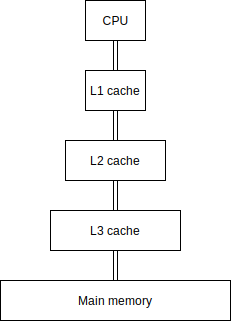
\includegraphics[width=0.4\textwidth,height=\textheight]{img/CacheLevels.pdf}
\caption{Illustration of cache levels in a typical system}
\end{figure}

If data is not already present in a cache layer, it is typically stored
there after it has been fetched from a slower cache level or main
memory. This is often a good decision to make as there's a high
likelihood the same address will be accessed by the program soon after.
This high likelihood is known as the
\href{https://en.wikipedia.org/wiki/Locality_of_reference}{principle of
locality}\index{principle
of locality}\index{locality of reference}.

Data is stored and transferred between cache levels in blocks of aligned
memory. Such a block is called a \textbf{cache block}\index{cache block}
or \textbf{cache line}\index{cache line}. Typical sizes are 32, 64 or
128 bytes per cache line.

When data that wasn't previously in the cache needs to be stored in the
cache, room has to be made for it by removing, or
\textbf{evicting}\index{cache eviction}, some other address/data from
it. How that choice gets made is decided by the
\href{https://en.wikipedia.org/wiki/Cache_replacement_policies}{cache
replacement policy}\index{cache
replacement policy}. Popular replacement algorithms are Least Recently
Used (LRU)\index{LRU replacement policy},
Random\index{random replacement policy} and
pseudo-LRU\index{pseudo-LRU replacement policy}. As the names suggest,
LRU evicts the cache line that is least recently used; random picks a
random cache line; and pseudo-LRU approximates choosing the least
recently used line.

If a cache line can be stored in all locations available in the cache,
the cache is \textbf{fully-associative}\index{fully-associative cache}.
Most caches are however not fully-associative, as it's too costly to
implement. Instead, most caches are
\textbf{set-associative}\index{set-associative cache}. In an N-way
set-associative cache, a specific line can only be stored in one of N
cache locations. For example, if a line can potentially be stored in one
of 2 locations, the cache is said to be 2-way set-associative. If it can
be stored in one of 4 locations, it's called 4-way set-associative, and
so on. When an address can only be stored in one location in the cache,
it is said to be \textbf{direct-mapped}\index{direct-mapped cache},
rather than 1-way set-associative. Typical organizations are
direct-mapped, 2-way, 4-way, 8-way, 16-way or 32-way set-associative.

The set of cache locations that a particular cache line can be stored at
is called a \textbf{cache set}\index{cache set}.

\hypertarget{indexing-in-a-set-associative-cache}{%
\subsubsection{Indexing in a set-associative
cache}\label{indexing-in-a-set-associative-cache}}

For some cache covert channels, it is essential to know exactly how a
memory address maps to a specific cache set.

\begin{figure}
\hypertarget{fig:cache-indexing}{%
\centering
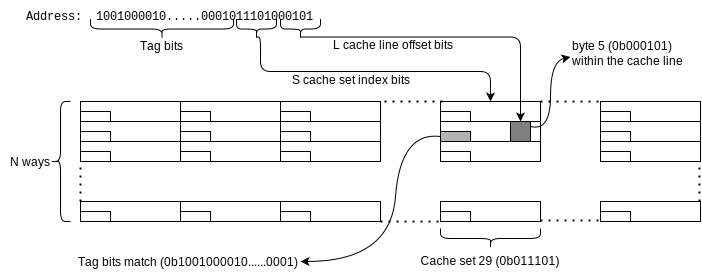
\includegraphics[width=1\textwidth,height=\textheight]{img/CacheIndexing.pdf}
\caption{Figure 5: Illustration of indexing into a set-associative
cache. In this example: \(L\) = 6 bits, hence the cache line size is
\(2^6=64\) bytes. \(S\) = 5 bits, so there are \(2^5=32\) cache sets.
\(N\) can be independent of address bits used to index the cache. If we
assume \(N=12\) for a 12-way set-associative cache, the total cache size
is \(N*2^L*2^S=12*64*32=24\)KB.}\label{fig:cache-indexing}
}
\end{figure}

Specific bits in the memory address are used for different cache
indexing purposes, as illustrated in figure
\protect\hyperlink{fig:cache-indexing}{5}. The least-significant \(L\)
bits, where \(2^L\) is the cache line size, are used to compute an
address's offset within a cache line. The next \(S\) bits, where \(2^S\)
is the number of cache sets, are used to determine which cache set an
address maps to. The remaining top bits are ``tag bits''. They are
stored alongside a line in the cache so later operations can detect
which specific memory address is replicated in that cache line.

For direct-mapped and fully-associative caches, the mapping of an
address to cache locations also works as described above. In
fully-associative caches the number of cache sets is 1, so \(S\)=0.

\tododiv{Also explain cache coherency \index{cache coherency}?
\href{https://github.com/llsoftsec/llsoftsecbook/issues/173}{\#173}}

\tododiv{Also say something about TLBs and prefetching?
\href{https://github.com/llsoftsec/llsoftsecbook/issues/174}{\#174}}

\hypertarget{operation-of-cache-side-channels}{%
\subsection{Operation of cache
side-channels}\label{operation-of-cache-side-channels}}

Cache side-channels typically work by the spy determining whether a
memory access was a cache hit or a cache miss. From that information,
the spy may be able to deduce bits of data that only the victim should
have access to.

Let's illustrate this by describing a few well-known cache
side-channels:

\hypertarget{flushreload}{%
\subsubsection{Flush+Reload}\label{flushreload}}

In a so-called \textbf{Flush+Reload}\index{Flush+Reload}
attack(\protect\hyperlink{ref-Yarom2014}{Yarom and Falkner 2014}), the
spy process shares memory with the victim process. The attack works in 3
steps:

\begin{enumerate}
\def\labelenumi{\arabic{enumi}.}
\tightlist
\item
  The Flush step: The spy flushes a specific address from the cache.
\item
  The spy waits for some time to give the victim time to potentially
  access that address, resulting in bringing it back into the cache.
\item
  The Reload step: The spy accesses the address and measures the access
  time. A short access time means the address is in the cache; a long
  access time means it's not in the cache. In other words, a short
  access time means that in step 2 the victim accessed the address; a
  long access time means it did not access the address.
\end{enumerate}

\tododiv{Should there be a more elaborate example with code that
demonstrates in more detail how a flush+reload attack works?
\href{https://github.com/llsoftsec/llsoftsecbook/issues/175}{\#175}}

Knowing if a victim accessed a specific address can leak sensitive
information. Such as when accessing a specific array element depends on
whether a specific bit is set in secret data. For example,
(\protect\hyperlink{ref-Yarom2014}{Yarom and Falkner 2014}) demonstrates
that a Flush+Reload attack can be used to leak GnuPG private keys.

\hypertarget{primeprobe}{%
\subsubsection{Prime+Probe}\label{primeprobe}}

In a \textbf{Prime+Probe} attack\index{Prime+Probe}, there is no need
for memory to be shared between victim and spy. The attack works in 3
steps:

\begin{enumerate}
\def\labelenumi{\arabic{enumi}.}
\tightlist
\item
  The Prime step: The spy fills one or more cache sets with its data,
  for example, by accessing data that maps to those cache sets.
\item
  The spy waits for some time to let the victim potentially access data
  that maps to those same cache sets.
\item
  The Probe step: The spy accesses that same data as in the prime step.
  Measuring the time it takes to load the data, it can derive how many
  cache lines the victim evicted from each cache set in step 2, and from
  that derive information about addresses the victim accessed.
\end{enumerate}

(\protect\hyperlink{ref-Osvik2005}{Osvik, Shamir, and Tromer 2005})
first documented this technique in 2005 and demonstrates extracting AES
keys in just a few milliseconds.

\hypertarget{general-schema-for-cache-covert-channels}{%
\subsubsection{General schema for cache covert
channels}\label{general-schema-for-cache-covert-channels}}

An attentive reader may have noticed that the attacks described above
follow a similar 3-step pattern.
(\protect\hyperlink{ref-Weber2021}{Weber et al. 2021}) describes this
general pattern and uses it to automatically discover more side-channels
that follow this 3-step pattern. They describe the general pattern as
being:

\begin{enumerate}
\def\labelenumi{\arabic{enumi}.}
\tightlist
\item
  An instruction sequence that resets the inner CPU state (\textbf{reset
  sequence}).\index{reset sequence}
\item
  An instruction sequence that triggers a state change (\textbf{trigger
  sequence}).\index{trigger sequence}
\item
  An instruction sequence that leaks the inner state
  (\textbf{measurement sequence}).\index{measurement sequence}
\end{enumerate}

Other cache-based side channel attacks following this general 3-step
approach include:
Flush+Flush\index{Flush+Flush}(\protect\hyperlink{ref-Gruss2016a}{Gruss,
Maurice, Wagner, et al. 2016}),
Flush+Prefetch\index{Flush+Prefetch}(\protect\hyperlink{ref-Gruss2016}{Gruss,
Maurice, Fogh, et al. 2016}),
Evict+Reload\index{Evict+Reload}(\protect\hyperlink{ref-Percival2005}{Percival
2005}),
Evict+Time\index{Evict+Time}(\protect\hyperlink{ref-Osvik2005}{Osvik,
Shamir, and Tromer 2005}),
Reload+Refresh\index{Reload+Refresh}(\protect\hyperlink{ref-Briongos2020}{Briongos
et al. 2020}),
Collide+Probe\index{Collide+Probe}(\protect\hyperlink{ref-Lipp2020}{Lipp
et al. 2020}), etc.

\hypertarget{mitigating-cache-side-channel-attacks}{%
\subsection{Mitigating cache side-channel
attacks}\label{mitigating-cache-side-channel-attacks}}

As described in (\protect\hyperlink{ref-Su2021}{Su and Zeng 2021}), 3
conditions need to be met for a cache-based side-channel attack to
succeed:

\begin{enumerate}
\def\labelenumi{\arabic{enumi}.}
\tightlist
\item
  There is a mapping between a state change in the cache and sensitive
  information in the victim program.
\item
  The spy runs on a CPU that shares a cache level with the CPU the
  victim runs on.
\item
  The spy can infer a cache status change caused by the victim through
  its own cache status.
\end{enumerate}

Mitigations against cache side-channel attacks can be categorized
according to which of the 3 conditions above they aim to prevent from
happening:

\hypertarget{mitigations-de-correlating-cache-state-change-with-sensitive-information-in-the-victim-program}{%
\subsubsection{Mitigations de-correlating cache state change with
sensitive information in the victim
program}\label{mitigations-de-correlating-cache-state-change-with-sensitive-information-in-the-victim-program}}

A typical example of when a cache state change could be correlated to
sensitive information is when a program uses secret information to index
into an array. An attacker could derive bits of the secret information
by observing which cache line was fetched.

Especially in crypto kernels, indexing into an array using a secret
value is generally avoided. An alternative mitigation is to always
access all array indices, independent of the secret value, e.g.~as done
in
\href{https://git.tartarus.org/?p=simon/putty.git;a=commitdiff;h=46fbe375bf}{commit
46fbe375} to the PuTTY project, which contains this comment:

\begin{quote}
\begin{verbatim}
* Side-channel considerations: the exponent is secret, so
* actually doing a single table lookup by using a chunk of
* exponent bits as an array index would be an obvious leak of
* secret information into the cache. So instead, in each
* iteration, we read _all_ the table entries, and do a sequence
* of mp_select operations to leave just the one we wanted in the
* variable
\end{verbatim}
\end{quote}

\hypertarget{mitigations-disallowing-spy-programs-to-share-the-cache-with-the-victim-program}{%
\subsubsection{Mitigations disallowing spy programs to share the cache
with the victim
program}\label{mitigations-disallowing-spy-programs-to-share-the-cache-with-the-victim-program}}

If the victim and the spy do not share a common channel -- in this case
a cache level -- then a side channel cannot be created.

One way to achieve this is to only allow one program to run at the same
time, and when a context switch does happen, to clear all cache content.
Obviously, this has a huge performance impact, especially in systems
with multiple cores and with large caches. Therefore, a wide variety of
mitigations have been proposed that aim to make attacks somewhat harder
without losing too much system efficiency.
(\protect\hyperlink{ref-Mushtaq2020}{Mushtaq et al. 2020}) and
(\protect\hyperlink{ref-Su2021}{Su and Zeng 2021}) summarize dozens of
proposals and implementations -- too many to try to describe them all
here.

One popular such mitigation is disabling
\href{https://en.wikipedia.org/wiki/Multithreading_(computer_architecture)}{cpu
multithreading}\index{multithreading}. For example,
\href{https://learn.microsoft.com/en-us/azure/virtual-machines/mitigate-se}{Azure
suggests that users who run untrusted code should consider disabling cpu
multithreading}.
\href{https://www.kernel.org/doc/Documentation/admin-guide/hw-vuln/core-scheduling.rst}{The
linux kernel's core scheduling documentation} also states mutually
untrusted code should not run on the same core concurrently. It
implements a scheduler that
\href{https://lwn.net/Articles/861251/}{takes into account which
processes are mutually-trusting} and only allows those to run
simultaneously on the same core.

One could argue that
\href{https://developer.chrome.com/blog/site-isolation/}{site
isolation}\index{site
isolation} as implemented in many web browsers is a mitigation that also
falls into this category. Site isolation is described in more detail in
\protect\hyperlink{site-isolation}{its own section}.

\hypertarget{mitigations-disabling-the-spy-program-to-infer-a-cache-status-change-in-the-victim-program-through-its-own-cache-status}{%
\subsubsection{Mitigations disabling the spy program to infer a cache
status change in the victim program through its own cache
status}\label{mitigations-disabling-the-spy-program-to-infer-a-cache-status-change-in-the-victim-program-through-its-own-cache-status}}

In some contexts, the resolution of the smallest time increment
measurable by the spy program can be reduced so much that it becomes
much harder to distinguish between a cache hit and a cache miss.
Injecting noise and jitter into the timer also makes it harder to
distinguish between a cache hit and cache miss. This is one of the
mitigations in javascript engines against Spectre attacks. For more
information see this \href{https://v8.dev/blog/spectre}{v8 blog post} or
this
\href{https://developer.mozilla.org/en-US/docs/Web/API/Performance/now}{Firefox
documentation of the performance.now() method}\index{Spectre}.

Note that this is not a perfect mitigation - there are often surprising
ways that an attacker can get a fine-grained enough timer or use
statistical methods to be able to detect the difference between a cache
hit or miss. One extreme example is the NetSpectre\index{NetSpectre}
attack (\protect\hyperlink{ref-Schwarz2019}{Schwarz et al. 2019}) where
the difference between cache hit and cache miss is measured over a
network, by statistically analyzing delays on network packet responses.
Furthermore, (\protect\hyperlink{ref-Schwarz2017}{Schwarz et al. 2017})
demonstrates how to construct high-resolution timers in various indirect
ways in all browsers that have removed explicit fine-grained timers.

Another possibility is to clear the cache between times when the victim
runs and the spy runs. This is probably going to incur quite a bit of
performance overhead, and may also not always possible e.g.~when victim
and spy are running at the same time on 2 CPUs sharing a cache level.

\hypertarget{branch-predictor-based-side-channels}{%
\section{Branch-predictor based
side-channels}\label{branch-predictor-based-side-channels}}

\hypertarget{branch-predictors}{%
\subsection{Branch predictors}\label{branch-predictors}}

Most CPUs implement one or more
\href{https://en.wikipedia.org/wiki/Instruction_pipelining}{instruction
pipelines}. \index{pipeline}\index{instruction pipeline} In an
instruction pipeline, the next instruction is started before the
previous instruction has finished executing. When the previous
instruction is a branch instruction, the next instruction that needs to
be executed is only known when that branch instruction completes.
However, waiting for the branch instruction to finish before starting
the next instruction leads to a big performance loss.\footnote{Over
  time, new CPU designs tend to support having more instructions in
  flight. (\protect\hyperlink{ref-Eyerman2009}{Eyerman et al. 2009, sec.
  4.2.3}) suggests that branch prediction accuracy has to grow more than
  linearly when the number of pipelines, or the depth of the pipeline
  grows. Therefore, there is a constant push to increase the accuracy of
  branch predictors.} Therefore, most CPUs predict\index{predict} which
instruction needs to be executed after a branch, before the branch
instruction has completed. Correctly and quickly predicting the
instruction after a branch instruction is so important for performance
that most CPUs have multiple
\href{https://en.wikipedia.org/wiki/Branch_predictor}{branch
predictors}\index{branch
predictor}, such as:

\begin{itemize}
\tightlist
\item
  A predictor of the outcome of a conditional
  branch\index{conditional branch
  direction predictor}: taken or not taken\index{taken branch}. The
  prediction is typically history-based\index{history-based prediction},
  i.e.~based on the outcome of this and other branches in the recent
  past.
\item
  A predictor of the target of a taken
  branch\index{branch target predictor}, i.e.~the address of the next
  instruction after a taken branch.
\item
  A predictor that is specialized to predict the next instruction after
  a function return instruction.\index{return address predictor}
\end{itemize}

\hypertarget{side-channels-through-branch-predictors}{%
\subsection{Side-channels through branch
predictors}\label{side-channels-through-branch-predictors}}

A number of attacks have been described over the past few years. The
following sections list a few examples, categorized per branch predictor
component they target.

\hypertarget{conditional-branch-direction-predictor-side-channel-attacks}{%
\subsubsection{Conditional branch direction predictor side-channel
attacks}\label{conditional-branch-direction-predictor-side-channel-attacks}}

\index{conditional branch direction predictor}

Two examples are BranchScope
(\protect\hyperlink{ref-Evtyushkin2018}{Evtyushkin et al.
2018})\index{BranchScope} and BlueThunder
(\protect\hyperlink{ref-Huo2019}{Huo et al. 2019})\index{BlueThunder}.
These attacks infer whether a branch is taken or not taken in a victim
process. They do so by carefully making sure that a branch in the spy
process uses the same branch predictor entry as the targeted branch in
the victim process. By measuring whether the branch in the spy process
gets predicted correctly, one can derive whether the branch in the
victim process was taken or not.

This can be thought of as somewhat akin to the
\protect\hyperlink{primeprobe}{Prime+Probe cache-based side channel
attacks}.

When the outcome of a branch depends on a bit in a secret key, this can
enable an attacker to derive the value of the secret key. These papers
demonstrate deriving the secret key from implementations of specific
cryptographic kernels. It can also be used to break
\protect\hyperlink{aslr}{ASLR}\index{ASLR}.

\hypertarget{branch-target-predictor-side-channel-attacks}{%
\subsubsection{Branch target predictor side-channel
attacks}\label{branch-target-predictor-side-channel-attacks}}

\index{Branch target predictor}

Two examples are SBPA (\protect\hyperlink{ref-Aciicmez2007}{Aciiçmez,
Kaya Koç, and Seifert 2007})\index{SBPA} and BranchShadow
(\protect\hyperlink{ref-Lee2017}{Lee et al. 2017})\index{BranchShadow}.
These earlier attacks are based on making a branch in the spy process
alias in the Branch Target Buffer (BTB\index{BTB}) with a targeted
branch in the victim process. They use methods such as timing
difference, last branch records\index{last branch record}, instruction
traces\index{instruction trace} or performance
counters\index{performance counter} to measure whether the branch in the
spy process caused a specific state change in the BTB.

\hypertarget{return-address-predictor-side-channel-attacks}{%
\subsubsection{Return address predictor side-channel
attacks}\label{return-address-predictor-side-channel-attacks}}

\index{return address predictor}

One example is Hyper-Channel
(\protect\hyperlink{ref-Bulygin2008}{Bulygin
2008})\index{Hyper-Channel}. In this case, a spy process invokes \(N\)
calls to fill up the return stack predictor. Then it lets the victim
process execute. Then, the spy process can measure how many of its
return stack entries have been removed from the Return Stack Buffer
(RSB), by measuring the number of \(N\) returns that get mis-predicted.
If the number of calls in the victim process is dependent on secret
information, this could leak it.

The papers referred to above contain detailed explanations of how they
set up the attack. All of these attacks use a general 3-step approach,
similar to
\protect\hyperlink{general-schema-for-cache-covert-channels}{cache side
channels}:

\begin{enumerate}
\def\labelenumi{\arabic{enumi}.}
\tightlist
\item
  An instruction sequence that resets the branch predictor state
  (\emph{reset sequence}), run by the spy process.\index{reset sequence}
\item
  An instruction sequence that triggers a branch predictor state change
  (\emph{trigger sequence}), run by the victim
  process.\index{trigger sequence}
\item
  An instruction sequence that leaks the branch predictor state
  (\emph{measurement sequence}), run by the spy
  process\index{measurement sequence}
\end{enumerate}

\hypertarget{mitigations}{%
\subsection{Mitigations}\label{mitigations}}

\tododiv{Describe the mitigations proposed against these side-channel
attacks.
\href{https://github.com/llsoftsec/llsoftsecbook/issues/203}{\#203}}

\hypertarget{resource-contention-channels}{%
\section{Resource contention
channels}\label{resource-contention-channels}}

\hypertarget{channels-making-use-of-aliasing-in-other-predictors}{%
\section{Channels making use of aliasing in other
predictors}\label{channels-making-use-of-aliasing-in-other-predictors}}

\tododiv{Should we also discuss more ``covert'' channels here such as
power analysis, etc?
\href{https://github.com/llsoftsec/llsoftsecbook/issues/176}{\#176}}

\hypertarget{transient-execution-attacks}{%
\section{Transient execution
attacks}\label{transient-execution-attacks}}

\hypertarget{transient-execution}{%
\subsection{Transient execution}\label{transient-execution}}

\hypertarget{speculative-execution}{%
\subsubsection{Speculative execution}\label{speculative-execution}}

CPUs execute sequences of instructions. There are often dependencies
between instructions in the sequence. That means that the outcome of one
instruction influences the execution of a later instruction.

Apart from the smallest micro-controllers, all CPUs execute multiple
instructions in parallel. Sometimes even multiple hundreds of them at
the same time, all in various stages of execution. Instructions start
executing while potentially hundreds of previous instructions haven't
produced their results yet. How can a CPU achieve this when the output
of a previous instruction, which might not have fully executed yet, and
hence whose output may not yet be ready, may affect the execution of
that later instruction? In other words, there may be a
\textbf{dependency} between an instruction that has not finished yet and
a later instruction that the CPU also already started executing.

There are various kinds of dependencies. One kind is \textbf{control
dependencies}\index{control dependencies}, where whether the later
instruction should be executed at all is dependent on the outcome of the
earlier instruction. Other kinds are \textbf{true data
dependencies}\index{true data
dependency}, \textbf{anti-dependencies}\index{anti dependency} and
\textbf{output dependencies}\index{output dependency}. More details
about these kinds of dependencies can be found on
\href{https://en.wikipedia.org/wiki/Data_dependency}{the wikipedia page
about them}.

CPUs overcome parallel execution limitations imposed by dependencies by
making massive numbers of \textbf{predictions}\index{prediction}. For
example, most CPUs predict whether conditional branches are taken or
not, which is making a prediction on control dependencies. Another
example is a CPU making a prediction on whether a load accesses the same
memory address as a preceding store. If they do not access the same
memory locations, the load can run in parallel with the store, as there
is no data dependency between them. If they do access overlapping memory
locations, there is a dependency and the store should complete before
the load can start executing.

Starting to execute later instructions before all of their dependencies
have been resolved, based on the predictions, is called
\textbf{speculation}\index{speculation}.

Let's illustrate that with an example. The following C code

\begin{Shaded}
\begin{Highlighting}[]
\DataTypeTok{long}\NormalTok{ abs}\OperatorTok{(}\DataTypeTok{long}\NormalTok{ a}\OperatorTok{)} \OperatorTok{\{}
  \ControlFlowTok{if} \OperatorTok{(}\NormalTok{a }\OperatorTok{\textgreater{}=} \DecValTok{0}\OperatorTok{)}
    \ControlFlowTok{return}\NormalTok{ a}\OperatorTok{;}
  \ControlFlowTok{else}
    \ControlFlowTok{return} \OperatorTok{{-}}\NormalTok{a}\OperatorTok{;}
\OperatorTok{\}}
\end{Highlighting}
\end{Shaded}

can be translated to the following AArch64 assembly code:

\begin{Shaded}
\begin{Highlighting}[]
        \BuiltInTok{cmp}\NormalTok{     x0}\OperatorTok{,} \OperatorTok{\#}\DecValTok{0}
\NormalTok{        b}\OperatorTok{.}\NormalTok{ge    Lbb2}
\FunctionTok{Lbb1:}
        \BuiltInTok{neg}\NormalTok{     x0}\OperatorTok{,}\NormalTok{ x0}
\FunctionTok{Lbb2:}
        \ControlFlowTok{ret}
\end{Highlighting}
\end{Shaded}

The \texttt{b.ge} instruction is a conditional branch instruction. It
computes whether the next instruction should be the one immediately
after, or the one pointed to by label \texttt{Lbb2}. In case it's the
instruction immediately after, the branch is said to not be taken.
Instead, if it's the instruction pointed to be label \texttt{Lbb2}, the
branch is said to be taken. When the condition \texttt{.ge} (greater or
equal) is true, the branch is taken. That condition is defined or set by
the previous instruction, the \texttt{cmp\ x0,\ \#0} instruction, which
compares the value in register \texttt{x0} with 0. Therefore, there is a
dependency between the \texttt{cmp} instruction and the \texttt{b.ge}
instruction. To overcome this dependency, and be able to execute the
\texttt{cmp}, \texttt{b.ge} and potentially more instructions in
parallel, the CPU predicts the outcome of the branch instruction. In
other words, it predicts whether the branch is taken or not. The CPU
will pick up either the \texttt{neg} or the \texttt{ret} instruction to
start executing next. This is called \emph{speculation}, as the CPU
\emph{speculatively executes} either instruction \texttt{neg}, or
\texttt{ret}.

\tododiv{Show a second example of cpu speculation that is not based on
branch prediction.
\href{https://github.com/llsoftsec/llsoftsecbook/issues/177}{\#177}}

Of course, as with all predictions, the CPU gets the prediction wrong
from time to time. In that case, all changes to the system state that
affect the correct execution of the program need to be undone. In the
above example, if the branch should have been taken, but the CPU
predicted it to not be taken, the \texttt{neg} instruction is executed
incorrectly and changes the value in register \texttt{x0}. After
discovering the branch was mis-predicted, the CPU would have to restore
the correct, non-negated, value in register \texttt{x0}.

Any instructions that are executed under so-called
\textbf{mis-speculation}\index{mis-speculation}, are called
\textbf{transient
instructions}\index{transient instructions}.\footnote{Transient
  instructions caused by incorrect branch-direction prediction have also
  been called \textbf{wrong-path
  instructions}\index{wrong-patch instructions} Mutlu et al.
  (\protect\hyperlink{ref-Mutlu2004}{2004})}

The paragraph above says ``\emph{the system state that affects the
correct execution of the program, needs to be undone}''. There is a lot
of system state that does not affect the correct execution of a program.
And the changes to such system state by transient instructions is often
not undone.

For example, a transient load instruction can fetch a value into the
cache that was not there before. By bringing that value in the cache, it
could have evicted another value from the cache. Whether a value is
present in the cache does not influence the correct execution of a
program; it merely influences its execution speed. Therefore, the effect
of transient execution on the content of the cache is typically not
undone when detecting mis-speculation.

Sometimes, it is said that the \textbf{architectural
effects}\index{architectural
effects} of transient instructions need to be undone, but the
\textbf{micro-architectural effects}\index{micro-architectural effects}
do not need to be undone.

The above explanation describes architectural effects as changes in
system state that need to be undone after detecting mis-speculation. In
reality, most systems will implement techniques that keep all state
changes in micro-architectural buffers until it is clear that all
predictions made to execute that instruction were correct. At that point
the micro-architectural state is \textbf{committed} to become
architectural state. In that way, mis-predictions naturally do not
affect architectural state. \todospan{{Could we find a good reference
that explains micro-architectural versus architectural state in more
detail? Is ``Computer Architecture: A Quantitative Approach'' the best
reference available?}}

\textbf{Faulting instructions}\index{faulting instructions} are
instructions that generate an exception at run-time. Many instructions
can generate an exception, and are hence \textbf{potentially faulting}.
For example most load and store instructions generate an exception when
the accessed address is not mapped. Since so many instructions can
generate an exception, processors typically speculate that they do not
generate an exception to enable more parallel execution.

When an instruction faults, the execution typically continues at another
location. Any instructions later in the instruction stream which are
speculatively executed before the fault is detected are also called
\textbf{transient instructions}\index{transient instructions}.

There is a kind of control dependency between every potentially-faulting
instruction and the next one, as the next instruction to be executed
depends on whether the instruction generates an exception or not. We
call out this dependency separately here as the transient execution
attacks we'll describe next get classified based on whether they make
use of transient instructions after a misprediction, or transient
instructions after a faulting instruction.

\hypertarget{transient-execution-attacks-1}{%
\subsection{Transient Execution
Attacks}\label{transient-execution-attacks-1}}

\textbf{Transient execution attacks}\index{transient execution attacks}
are a category of side-channel attacks that use the micro-architectural
side-effects of transient execution as a side channel.

The publication of the Spectre\index{Spectre}
(\protect\hyperlink{ref-Kocher2019}{Kocher et al. 2019}) and
Meltdown\index{Meltdown} (\protect\hyperlink{ref-Lipp2018}{Lipp et al.
2018}) attacks in 2018 started a period in which a large number of
transient attacks were discovered and published. Most of them were given
specific names, such as ZombieLoad, NetSpectre, LVI, Straight-line
Speculation, etc. New variants continue to be published regularly.

Covering each one of them in detail here would make the book overly
lengthy, and may not necessarily help much with gaining a better insight
in the common characteristics of transient attacks. Therefore, we'll try
to put them into a few categories and describe the characteristics of
each category.

\tododiv{Decide whether it's useful to talk about alternative
categorizations of transient execution attacks, and if so, do add
content. Consider pointing to
\url{https://github.com/MattPD/cpplinks/blob/master/comparch.micro.channels.md}}

The categorization below is based on one proposed in
(\protect\hyperlink{ref-Bulck2020}{Bulck et al., n.d.}). There are
alternative categorizations. (\protect\hyperlink{ref-Bulck2020}{Bulck et
al., n.d.}) defines 4 big classes of transient side-channel attack
categories, based on whether:

\begin{enumerate}
\def\labelenumi{\arabic{enumi}.}
\tightlist
\item
  The transient execution happens because of a misprediction, or a
  faulting instruction.
\item
  The attacker actively steers data or control flow of the transient
  execution or not.
\end{enumerate}

This gives the following 4 categories:

\begin{longtable}[]{@{}
  >{\raggedright\arraybackslash}p{(\columnwidth - 4\tabcolsep) * \real{0.2361}}
  >{\raggedright\arraybackslash}p{(\columnwidth - 4\tabcolsep) * \real{0.3611}}
  >{\raggedright\arraybackslash}p{(\columnwidth - 4\tabcolsep) * \real{0.3472}}@{}}
\toprule\noalign{}
\multirow{2}{*}{\begin{minipage}[b]{\linewidth}\raggedright
\end{minipage}} & \multicolumn{2}{l@{}}{%
\begin{minipage}[b]{\linewidth}\raggedright
Steering of transient execution by attacker?
\end{minipage}} \\
& \begin{minipage}[b]{\linewidth}\raggedright
No (Leakage)
\end{minipage} & \begin{minipage}[b]{\linewidth}\raggedright
Yes (Injection)
\end{minipage} \\
\midrule\noalign{}
\endhead
\bottomrule\noalign{}
\endlastfoot
Misprediction & Branch-predictor based side-channels & Spectre-style
attacks \\
Faulting & Meltdown-style attacks & LVI-style attacks \\
\end{longtable}

\hypertarget{branch-predictor-based-side-channel-attacks}{%
\subsubsection{Branch predictor-based side-channel
attacks}\label{branch-predictor-based-side-channel-attacks}}

We discussed this category already in the section on
\protect\hyperlink{side-channels-through-branch-predictors}{Side-channels
through branch predictors}.

\hypertarget{spectre-style-attacks}{%
\subsubsection{Spectre-style attacks}\label{spectre-style-attacks}}

\tododiv{Add a description of Spectre-style attacks such as Spectre-PHT,
Spectre-BTB, Spectre-RSB, Spectre-STL, SpectreV1, SpectreV2, SpectreV3,
SpectreV4, NetSpectre.
\href{https://github.com/llsoftsec/llsoftsecbook/issues/178}{\#178}}

\hypertarget{meltdown-style-attacks}{%
\subsubsection{Meltdown-style attacks}\label{meltdown-style-attacks}}

\tododiv{Add a description of Meltdown-style attacks such as Meltdown,
Foreshadow, LazyFP, Fallout, ZombieLoad, RIDL.
\href{https://github.com/llsoftsec/llsoftsecbook/issues/178}{\#178}}

\hypertarget{lvi-style-attacks}{%
\subsubsection{LVI-style attacks}\label{lvi-style-attacks}}

\tododiv{Add a description of LVI-style attacks.
\href{https://github.com/llsoftsec/llsoftsecbook/issues/178}{\#178}}

\hypertarget{mitigations-against-transient-execution-attacks}{%
\subsection{Mitigations against transient execution
attacks}\label{mitigations-against-transient-execution-attacks}}

\hypertarget{site-isolation}{%
\subsubsection{Site isolation}\label{site-isolation}}

\tododiv{Write section on site isolation as a SpectreV1 mitigation
\href{https://github.com/llsoftsec/llsoftsecbook/issues/179}{\#179}}

\hypertarget{physical-access-side-channel-attacks}{%
\section{Physical access side-channel
attacks}\label{physical-access-side-channel-attacks}}

\hypertarget{supply-chain-attacks}{%
\chapter{Supply chain attacks}\label{supply-chain-attacks}}

A software \emph{supply chain attack} occurs when an attacker interferes
with the software development or distribution processes with the
intention to impact users of that software.

Supply chain attacks and their possible mitigations are not specific to
compilers. However, compilers are an attractive target for attack
because they are widely deployed to developers, in continuous
integration systems and as JITs. Also, an infected compiler has the
possibility to make a much larger impact if it can silently spread the
infection to other software created with or run using it.

This chapter explores the history of supply chain attacks that involve
compilers and what can be done to prevent them.

\hypertarget{history-of-supply-chain-attacks}{%
\section{History of supply chain
attacks}\label{history-of-supply-chain-attacks}}

As far back as 1974 Karger \& Schell theorized about an attack on the
Multics operating system via the PL/I compiler
(\protect\hyperlink{ref-Karger1974}{Paul A. and Roger R. 1974}). In this
attack, a trap door is inserted into the compiler, which then injects
malicious code into generated object code. Furthermore, the trap door
could be designed to reinsert itself into the compiler binary so that
future compilers are silently infected without needing changes to their
source code. This attack method was subsequently popularized by Ken
Thompson in his 1984 ACM Turing Award acceptance speech
\emph{Reflections on Trusting Trust}
(\protect\hyperlink{ref-Thompson1984}{Thompson 1984}).

If these cases seem far-fetched then consider that there have been
several real examples of supply chain attacks on development tools.

Induc is a family of viruses that infects a pre-compiled library in the
Delphi toolchain with malicious code
(\protect\hyperlink{ref-Gostev2009}{Gostev 2009}). When Delphi compiles
a project the malicious library is included into the resulting
executable, thus enabling the virus to spread. The virus was first
detected in 2009 and was circulating undetected for at least a year
beforehand. Several popular applications are known to have been
infected, including a chat client and a media player. Overall, in excess
of a hundred thousand infected computers were detected world-wide by
anti-virus solutions.

XcodeGhost is the name given to malware first detected in 2015 that
infected thousands of iOS applications
(\protect\hyperlink{ref-Cox2015}{Cox 2015}). The source of the infection
was tracked down to a trojanized version of Xcode tools. The malware
exists in an extra object file within the Xcode tools and is silently
linked into each application as it is built. File sharing sites were
used to spread the trojanized Xcode tools to unwitting developers.

A trojanized linker was found to be involved in a supply chain attack
discovered in 2017 named ShadowPad
(\protect\hyperlink{ref-Greenberg2019}{Greenberg 2019}). Some instances
of the attack were perpetrated using a trojanized Visual Studio linker
that silently incorporates a malicious library into applications as they
are built. Related attacks named CCleaner and ShadowHammer used the same
approach of a trojanized linker to infect built applications. Infected
applications from these attacks were distributed to millions of users
world-wide.

These cases highlight that attacks on compilers, and especially linkers
and libraries, are a viable route to silently infect many other
applications, and there is no doubt that there will be more such attacks
in the future. Let us now explore what we can do about these.

\tododiv{Explain how these vulnerabilities arise and how to mitigate
them.
\href{https://github.com/llsoftsec/llsoftsecbook/issues/180}{\#180}}

\hypertarget{compiler-introduced-security-vulnerabilities}{%
\chapter{Compiler introduced security
vulnerabilities}\label{compiler-introduced-security-vulnerabilities}}

Security vulnerabilities introduced by compilers have a long history.
Thompson (\protect\hyperlink{ref-Thompson1984}{Thompson 1984}) provides
one of the oldest and most popular examples in this area. In his paper,
he talks about a compiler that can detect when it is compiling the login
program and can insert a backdoor so that he can use the system as any
user. However most common cases are where involuntary security
vulnerabilities are added in the generated binary by the compiler.

\tododiv{Explain how code that results in undefined behaviour can often
work as the programmer expected until some optimisation is applied, and
perhaps even talk a bit about why compilers rely on the absence of
undefined behaviour in ways that appear aggressive in some occasions.
\href{https://github.com/llsoftsec/llsoftsecbook/issues/202}{\#202}}

When discussing compiler introduced security vulnerabilities, undefined
behavior plays a major role. Its implications were thoroughly discussed
by various works such as (\protect\hyperlink{ref-wang2012undefined}{Wang
et al. 2012}) (\protect\hyperlink{ref-d2015correctness}{D'Silva, Payer,
and Song 2015}) (\protect\hyperlink{ref-dusilent}{Du, Wu, and Mao,
n.d.}). By reading the works of these authors, one can see that even
projects that went through careful testing, such as Linux, FreeBSD or
PostgreSQL, could not escape from this class of vulnerabilities. To
better understand them, this chapter contains several examples of such
vulnerabilities, their implications and how they got fixed.

The first example is a 15 years old vulnerability that affected the
random number generator (RNG) in Mac OS X
(\protect\hyperlink{ref-Wang2015}{Wang 2015}). At some point in the
past, this vulnerability affected all *BSD operating systems, as they
have a common ancestor with Mac OS.

In the random number generator of the system, more specifically in
\texttt{srandomdev(3)}, we can spot the following piece of code used in
the seeding logic:

\begin{Shaded}
\begin{Highlighting}[]
\KeywordTok{struct}\NormalTok{ timeval tv}\OperatorTok{;}
\DataTypeTok{unsigned} \DataTypeTok{long}\NormalTok{ junk}\OperatorTok{;}

\NormalTok{gettimeofday}\OperatorTok{(\&}\NormalTok{tv}\OperatorTok{,}\NormalTok{ NULL}\OperatorTok{);}
\NormalTok{srandom}\OperatorTok{((}\NormalTok{getpid}\OperatorTok{()} \OperatorTok{\textless{}\textless{}} \DecValTok{16}\OperatorTok{)} \OperatorTok{\^{}}\NormalTok{ tv}\OperatorTok{.}\NormalTok{tv\_sec }\OperatorTok{\^{}}\NormalTok{ tv}\OperatorTok{.}\NormalTok{tv\_usec }\OperatorTok{\^{}}\NormalTok{ junk}\OperatorTok{);}
\end{Highlighting}
\end{Shaded}

For generating a seed for the RNG, the code uses the current time and an
uninitialized value from the stack, i.e.~\texttt{junk}. This triggers
undefined behavior as the C standard has no clear semantics for
uninitialized loads. Because of that, there was a huge difference in the
generated assembly code for two different Mac OS X releases.

In Mac OS X 10.6 the generated code looked like this:

\begin{Shaded}
\begin{Highlighting}[]
\NormalTok{leaq    }\BaseNTok{0xe0}\OperatorTok{(\%}\KeywordTok{rbp}\OperatorTok{),\%}\KeywordTok{rdi}
\NormalTok{xorl    }\OperatorTok{\%}\KeywordTok{esi}\OperatorTok{,\%}\KeywordTok{esi}
\NormalTok{callq   }\BaseNTok{0x001422ca}      \CommentTok{; symbol stub for: \_gettimeofday}
\NormalTok{callq   }\BaseNTok{0x00142270}      \CommentTok{; symbol stub for: \_getpid}
\BuiltInTok{movq}    \BaseNTok{0xe0}\OperatorTok{(\%}\KeywordTok{rbp}\OperatorTok{),\%}\KeywordTok{rdx}
\NormalTok{movl    }\BaseNTok{0xe8}\OperatorTok{(\%}\KeywordTok{rbp}\OperatorTok{),\%}\KeywordTok{edi}
\NormalTok{xorl    }\OperatorTok{\%}\KeywordTok{edx}\OperatorTok{,\%}\KeywordTok{edi}
\NormalTok{shll    }\OperatorTok{$}\BaseNTok{0}\NormalTok{x10}\OperatorTok{,\%}\KeywordTok{eax}
\NormalTok{xorl    }\OperatorTok{\%}\KeywordTok{eax}\OperatorTok{,\%}\KeywordTok{edi}
\NormalTok{xorl    }\OperatorTok{\%}\KeywordTok{ebx}\OperatorTok{,\%}\KeywordTok{edi}
\NormalTok{callq   }\BaseNTok{0x00142d68}      \CommentTok{; symbol stub for: \_srandom}
\end{Highlighting}
\end{Shaded}

While for Mac OS X 10.7 the code looked like this:

\begin{Shaded}
\begin{Highlighting}[]
\NormalTok{leaq    }\BaseNTok{0xd8}\OperatorTok{(\%}\KeywordTok{rbp}\OperatorTok{),\%}\KeywordTok{rdi}
\NormalTok{xorl    }\OperatorTok{\%}\KeywordTok{esi}\OperatorTok{,\%}\KeywordTok{esi}
\NormalTok{callq   }\BaseNTok{0x000a427e}      \CommentTok{; symbol stub for: \_gettimeofday}
\NormalTok{callq   }\BaseNTok{0x000a3882}      \CommentTok{; symbol stub for: \_getpid}
\NormalTok{callq   }\BaseNTok{0x000a4752}      \CommentTok{; symbol stub for: \_srandom}
\end{Highlighting}
\end{Shaded}

In the shorter version of the generated assembly code, the compiler
dropped the whole argument of \texttt{srandom} as an optimization. While
the optimised code respects the standard, it leaves room for an attacker
to exploit the system because the seed of the RNG can now be predicted.

In the meantime, this problem has been resolved in FreeBSD
(\protect\hyperlink{ref-FbsdJunk}{{``FreeBSD Mitigation for Srandom
Undefined Behavior''} 2012}) and OpenBSD
(\protect\hyperlink{ref-ObsdJunk}{{``OpenBSD Mitigation for Srandom
Undefined Behavior''} 2002}).

Current solutions for detecting this class of vulnerabilities include
LLVM's MemorySanitizer and Valgrind.

The next example covers a new type of undefined behavior that can easily
introduce security vulnerabilities. This time we talk about
dereferencing NULL pointers and what might go wrong with this operation.
The following piece of code is taken from Linux and introduces a
vulnerability by dereferencing the \texttt{tun} pointer before it checks
that the pointer is valid:

\begin{Shaded}
\begin{Highlighting}[]
\DataTypeTok{unsigned} \DataTypeTok{int}
\NormalTok{tun\_chr\_poll}\OperatorTok{(}\KeywordTok{struct}\NormalTok{ file }\OperatorTok{*}\NormalTok{file}\OperatorTok{,}\NormalTok{ poll\_table }\OperatorTok{*}\NormalTok{ wait}\OperatorTok{)}
\OperatorTok{\{}
  \KeywordTok{struct}\NormalTok{ tun\_file }\OperatorTok{*}\NormalTok{tfile }\OperatorTok{=}\NormalTok{ file}\OperatorTok{{-}\textgreater{}}\NormalTok{private\_data}\OperatorTok{;}
  \KeywordTok{struct}\NormalTok{ tun\_struct }\OperatorTok{*}\NormalTok{tun }\OperatorTok{=}\NormalTok{ \_\_tun\_get}\OperatorTok{(}\NormalTok{tfile}\OperatorTok{);}
  \KeywordTok{struct}\NormalTok{ sock }\OperatorTok{*}\NormalTok{sk }\OperatorTok{=}\NormalTok{ tun}\OperatorTok{{-}\textgreater{}}\NormalTok{sk}\OperatorTok{;}
  \ControlFlowTok{if} \OperatorTok{(!}\NormalTok{tun}\OperatorTok{)}
    \ControlFlowTok{return}\NormalTok{ POLLERR}\OperatorTok{;}
  \OperatorTok{...}
\OperatorTok{\}}
\end{Highlighting}
\end{Shaded}

Normally, this would cause a crash in the kernel or the function would
return POLLERR if address 0 was mapped in the address space. However the
compiler assumes that \texttt{tun} is a valid pointer when the execution
reaches the if statement. This happens because it saw an earlier
dereference just before the if statement. In this situation, the check
is considered redundant and deleted from the final binary. This allows
an attacker to continue executing code from \texttt{tun\_chr\_poll} when
address 0 is mapped.

To mitigate against this situation, GCC developers added a flag called
\texttt{-fno-delete-null-pointer-checks} that Linux integrated in its
compiler configuration.

Linux was not the only project that suffered from this problem. Chromium
(\protect\hyperlink{ref-ChromiumIssue}{{``Issue 3782: V8 Is Not
-Fsanitize=null Clean''} 2014}) and Mozilla
(\protect\hyperlink{ref-MozillaIssue}{{``GCC6 - TB Crashes Due to
Removed Null Pointer Checks for "This"''} 2016}) had problems in the
past with this.

There are also cases of security vulnerabilities that are not introduced
by undefined behavior, the following piece of code is such an example.
This was taken from the Linux kernel. Because the compiler sees that the
pointer hash is never used after this point, it decides to delete the
memset operation. We call this dead store optimization (DSO)
\index{dead store optimization}. This has serious security implications
because the intention of the programmer was to delete the \texttt{hash}
information from memory.

\begin{Shaded}
\begin{Highlighting}[]
\DataTypeTok{static} \DataTypeTok{void}\NormalTok{ extract\_buf}\OperatorTok{(}\KeywordTok{struct}\NormalTok{ entropy\_store }\OperatorTok{*}\NormalTok{r}\OperatorTok{,}\NormalTok{ \_\_u8 }\OperatorTok{*}\NormalTok{out}\OperatorTok{)} \OperatorTok{\{}
  \OperatorTok{...}
  \OperatorTok{{-}}\NormalTok{ memset}\OperatorTok{(\&}\NormalTok{hash}\OperatorTok{,} \DecValTok{0}\OperatorTok{,} \KeywordTok{sizeof}\OperatorTok{(}\NormalTok{hash}\OperatorTok{));}
  \OperatorTok{+}\NormalTok{ memzero\_explicit}\OperatorTok{(\&}\NormalTok{hash}\OperatorTok{,} \KeywordTok{sizeof}\OperatorTok{(}\NormalTok{hash}\OperatorTok{));}
\OperatorTok{\}}
\end{Highlighting}
\end{Shaded}

The solution Linux came with was to add a new function called
\texttt{memzero\_explicit} which under the hood looks like this:

\begin{Shaded}
\begin{Highlighting}[]
\DataTypeTok{void}\NormalTok{ memzero\_explicit}\OperatorTok{(}\DataTypeTok{void} \OperatorTok{*}\NormalTok{s}\OperatorTok{,} \DataTypeTok{size\_t}\NormalTok{ count}\OperatorTok{)}
\OperatorTok{\{}
\NormalTok{  memset}\OperatorTok{(}\NormalTok{s}\OperatorTok{,} \DecValTok{0}\OperatorTok{,}\NormalTok{ count}\OperatorTok{);}
\NormalTok{  OPTIMIZER\_HIDE\_VAR}\OperatorTok{(}\NormalTok{s}\OperatorTok{);}
\OperatorTok{\}}
\end{Highlighting}
\end{Shaded}

It still uses \texttt{memset} \index{memset} to delete the associated
security sensitive data, but it also tries to eliminate the risk of DSO
by using the OPTIMIZER\_HIDE\_VAR macro. This, however, is not enough to
fully eliminate dead stores
(\protect\hyperlink{ref-MemZeroBarrier}{{``Lib: Memzero\_explicit: Use
Barrier Instead of {OPTIMIZER\_HIDE\_VAR}''} 2015}). In case of using
LTO, the buffer \texttt{s} is still vulnerable. For this reason, Linux
maintainers added a further hardening mechanism by using a compiler
barrier instead:

\begin{Shaded}
\begin{Highlighting}[]
\DataTypeTok{void}\NormalTok{ memzero\_explicit}\OperatorTok{(}\DataTypeTok{void} \OperatorTok{*}\NormalTok{s}\OperatorTok{,} \DataTypeTok{size\_t}\NormalTok{ count}\OperatorTok{)}
\OperatorTok{\{}
\NormalTok{  memset}\OperatorTok{(}\NormalTok{s}\OperatorTok{,} \DecValTok{0}\OperatorTok{,}\NormalTok{ count}\OperatorTok{);}
  \OperatorTok{{-}}\NormalTok{ OPTIMIZER\_HIDE\_VAR}\OperatorTok{(}\NormalTok{s}\OperatorTok{);}
  \OperatorTok{+}\NormalTok{ barrier}\OperatorTok{();}
\OperatorTok{\}}
\end{Highlighting}
\end{Shaded}

There is still room for improvement regarding the introduced barrier
(\protect\hyperlink{ref-MemZeroDataBarrier}{{``Lib: Make
Memzero\_explicit More Robust Against Dead Store Elimination''} 2015}).
If the content of the buffer is present in registers, then the compiler
blindly proves again that the DSO can be triggered and the
\texttt{memset} will be again deleted. To mitigate against this, the
following patch was proposed:

\begin{Shaded}
\begin{Highlighting}[]
\OperatorTok{+}\NormalTok{ \#define barrier\_data}\OperatorTok{(}\NormalTok{ptr}\OperatorTok{)}\NormalTok{ \textbackslash{}}
\OperatorTok{+}\NormalTok{  \_\_asm\_\_ \_\_volatile\_\_}\OperatorTok{(}\StringTok{""}\OperatorTok{:} \OperatorTok{:}\StringTok{"r"}\OperatorTok{(}\NormalTok{ptr}\OperatorTok{)} \OperatorTok{:}\StringTok{"memory"}\OperatorTok{)}

\DataTypeTok{void}\NormalTok{ memzero\_explicit}\OperatorTok{(}\DataTypeTok{void} \OperatorTok{*}\NormalTok{s}\OperatorTok{,} \DataTypeTok{size\_t}\NormalTok{ count}\OperatorTok{)}
\OperatorTok{\{}
\NormalTok{  memset}\OperatorTok{(}\NormalTok{s}\OperatorTok{,} \DecValTok{0}\OperatorTok{,}\NormalTok{ count}\OperatorTok{);}
  \OperatorTok{{-}}\NormalTok{ barrier}\OperatorTok{();}
  \OperatorTok{+}\NormalTok{ barrier\_data}\OperatorTok{(}\NormalTok{s}\OperatorTok{);}
\OperatorTok{\}}
\end{Highlighting}
\end{Shaded}

In this patch we create a new barrier that will be guaranted to put the
content of the buffer in memory so that DSO can take no further effect.

Similar efforts were conducted in other projects such as OpenSSL
(\protect\hyperlink{ref-OpenSSLMemClr}{{``Lib: Make Memzero\_explicit
More Robust Against Dead Store Elimination''} 2016}). The approach
OpenSSL used is rather different but it achieves the same end goal,
i.e.~eliminating the effect of DSO. By making \texttt{memset\_func} a
volatile pointer to the actual implementation of \texttt{memset}, the
compiler is forced to dereference the pointer to get to the actual
\texttt{memset}, thus eliminating the risk of optimizing it out.

The C23 committee decided to tackle this problem from another angle,
i.e.~by adding a library function called \texttt{memset\_explicit}
(\protect\hyperlink{ref-MemSetProposal}{{``Memset\_explicit''} 2021}).
This function requires the compiler to not optimize the memory overwrite
away. However it is not trivial to implement such a functionality, as
GNU presents in (\protect\hyperlink{ref-GNUMemSet}{{``10.604
Memset\_explicit,''} n.d.}). The information may be present somewhere in
the machine, even if it was erased from memory.

\hypertarget{underhanded-code}{%
\chapter{Underhanded code}\label{underhanded-code}}

\textbf{Underhanded code} is code that looks like it is doing one thing
but actually does something else. It usually refers to code nefariously
written in this way to sneak malicious behavior not obviously visible on
code inspection. However the same applies also when the underhanded
behavior has been added by mistake - in fact the ideal attack would also
give the attacker the possibility to say it was an honest mistake.

(\protect\hyperlink{ref-Wheeler2020}{Wheeler 2020}) provides a more
systematic view of underhanded code than is given here. This chapter
presents some examples to give an overview of the attack and how a
compiler can (and can't) help, although this probably doesn't classify
as ``low level'' software security.

\hypertarget{assignment-and-equality-confusion}{%
\section{Assignment and equality
confusion}\label{assignment-and-equality-confusion}}

Probably the most classic example of underhanded code in C-style
languages is code that takes advantage of the fact that the assignment
(\texttt{=}) and the equality operator (\texttt{==}) look very similar.

\begin{verbatim}
void somefunction(UserPermissionLevel permission_level) {

   if (permission_level = LEVEL_ADMIN) {
       do_admin_action();
       return;
   }
   report_access_violation();
}
\end{verbatim}

Here \texttt{permission\_level} is not compared to
\texttt{LEVEL\_ADMIN}, but rather assigned that value. Meaning that if
\texttt{LEVEL\_ADMIN} is a non-zero value the if condition will evaluate
to true.

Both Clang and GCC detects this example with warning option
\texttt{-Wparentheses}. Adding a pair of parentheses around the
assignment silences that warning. Those extra parentheses would probably
draw a reviewer's attention in this specific example but had the
condition been more complex with multiple subexpressions combined with
\texttt{\textbar{}\textbar{}} and \texttt{\&\&} the parentheses had
looked normal.

This could be written off as a language design problem. Traditionally
Python has not supported using assignment as expressions, effectively
sidestepping this particular problem. When assignment expressions were
added to the language (\protect\hyperlink{ref-pep572}{Angelico, Peters,
and Rossum 2018}) (in python 3.8) the more visually distinct ``walrus
operator'' \texttt{:=} was used to avoid this risk of confusing with the
comparison operator. Even in cases where it is an existing language the
compiler can provide options to forbid risky constructs for those who
want and can opt in to it, essentially creating a new language that is a
subset of the original language.

\hypertarget{goto-fail}{%
\section{goto fail}\label{goto-fail}}

The ``goto-fail'' bug, officially known as
\href{https://nvd.nist.gov/vuln/detail/CVE-2014-1266}{CVE-2014-1266},
caused Apple devices to not correctly validate certificates in TLS
connections. It effectively disables the verification the function is
supposed to do, and is easy to miss in code review. This was most likely
a mistake that was not added intentionally, but still has the
characteristics of underhanded code.

The bug was caused by a duplicated ``goto fail'' line, which was
indented making it look like it was guarded by previous if clause, when
it in fact always was executed. Since the \texttt{err} variable was set
to 0 (i.e no error) inside the if, the function would always return 0.

\begin{verbatim}
OSStatus
SSLVerifySignedServerKeyExchange(...)
{
    OSStatus err;
    ...

    if ((err = SSLHashSHA1.update(&hashCtx, &serverRandom)) != 0)
        goto fail;
    if ((err = SSLHashSHA1.update(&hashCtx, &signedParams)) != 0)
        goto fail;
        goto fail;
    if ((err = SSLHashSHA1.final(&hashCtx, &hashOut)) != 0)
        goto fail;
    ...

fail:
    return err;
}
\end{verbatim}

At the time of the bug they didn't but nowadays both GCC and Clang have
a \texttt{-Wmisleading-indentation} option that detects this kind
problem.

Also automatic code formatting tools such as clang-format would help
finding this issue as it will fix the misleading indentation.

\hypertarget{trojan-source}{%
\section{Trojan Source}\label{trojan-source}}

``Trojan Source'' attacks described by
(\protect\hyperlink{ref-Boucher2023}{Boucher and Anderson 2023}) is
another way underhanded code could be achieved by doing something that
makes the editor (or other thing that displays code to the user) render
the code in a different way than the compiler parses it.

This is done by using unicode features. Support for bidirectional text
is one such feature, where it has special characters to mark regions of
text to be right-to-left or left-to-right to allow mixing e.g Arabic and
English in the same document. If these are used in cunning ways they can
make the text render in a way that makes a word look like it is
\emph{inside} a comment but to the compiler, which parses it in the
order it appears in the file, sees it is \emph{after} the comment.

GCC provides
\href{https://gcc.gnu.org/onlinedocs/gcc/Warning-Options.html\#index-Wbidi-chars_003d}{\texttt{-Wbidi-chars}}
to detect usage of writing direction markers. Clang compiler
\href{https://bugs.chromium.org/p/llvm/issues/detail?id=11\#c9}{doesn't}
provide such warning, but has a check in
\href{https://clang.llvm.org/extra/clang-tidy/checks/misc/misleading-bidirectional.html}{clang-tidy}

Another variant of ``trojan source'' is usage of homoglyphs, different
characters that looks similar or even identical (depending on font). As
an example, unicode contains the character ``Division Slash'' (U+2215)
which is different from the ordinary ascii slash ``Solidus'' (U+002F).

\begin{verbatim}
/* Important comment */
check_permissions();
/* Another comment */
\end{verbatim}

If the final slash on the first line isn't a slash but another similarly
looking character that the compiler doesn't understand as end of comment
it means that the whole snippet is commented out.

\hypertarget{physical-attacks}{%
\chapter{Physical attacks}\label{physical-attacks}}

\tododiv{This chapter should probably be moved under section `Physical
access side-channel attacks' higher-up
\href{https://github.com/llsoftsec/llsoftsecbook/issues/181}{\#181}}

\hypertarget{overview}{%
\section{Overview}\label{overview}}

There are many types of physical attacks -- these attack methods focus
on one or multiple physical properties of systems ( e.g.~CPU, GPU,
crypto hardware), and can either be

\begin{itemize}
\tightlist
\item
  Passive -- just monitoring physical quantities (e.g.~side channel
  information leakage), or
\item
  Active -- modification of physical quantities, for example, by

  \begin{itemize}
  \tightlist
  \item
    changing the operation conditions of the system so that the circuit
    operates outside its specifications (e.g.~by changing temperature,
    or by applying glitches to supply voltage/clock source)
  \item
    injecting faults to the system (e.g.~altering the electrical state
    of the system using Electromagnetic pulse injection, or laser beam)
  \item
    physically modifying the system/chip
  \end{itemize}
\end{itemize}

In the rest of this section, we will focus on a subset of physical
attacks:

\begin{itemize}
\tightlist
\item
  Side channel information leakage
\item
  Physical attack using glitches
\end{itemize}

These two forms of attacks can be carried out using low cost hardware,
and have been widely demonstrated by researchers on SoCs or
microcontrollers developed for IoT (Internet-of-Things) applications.

\hypertarget{physical-access-side-channel-attacks-1}{%
\section{Physical access side-channel
attacks}\label{physical-access-side-channel-attacks-1}}

If an attacker has physical access to a device, even without debug
access, the attacker can collect side channel information about the
program execution on a processor. If the processor is used to handle
cryptographic operations, the side channel information can be used to
deduce the crypto key(s) or the data being processed. Please note that
some forms of physical attacks (e.g.~fault injection attacks like
rowhammer and voltjockey) do not require physical access, but those
attacks are not covered in this section.

\hypertarget{how-is-information-leaked}{%
\subsection{How is information
leaked?}\label{how-is-information-leaked}}

The most common physical access side channel attack method is to capture
the voltage or current consumption of the device during its operation.
Every time a flip-flop toggles, the switching activity results in a
small current spike. Even though there is capacitance on the power
distribution connections inside the chip, the toggling of registers
(composed of flip-flops) still results in variations in the power supply
current, which can be observed easily. Because the connections for
delivering power (at the power supply, printed circuit board, on chip
packages as well as on the silicon dies) also contain resistance, the
variation of electrical current in the chip's power supply also results
in variations in the power supply voltage. Again, this can be observed
easily if the attacker has physical access to the device. If an attacker
has access to data acquisition equipment that can record the
current/voltage/power patterns, he/she can record the ``power
signature'' for different crypto operations, including the power
signature using different data inputs. By applying analysis techniques
like differential power analysis, the attacker can extract the
information being processed. One additional form of side-channel leakage
is electro-magnetic radiation. Because the processor's clock frequency
is usually in the radio frequency (RF) range, the wires on the die and
the tracks on the PCB become small antennas, and the ripples in the
processor's voltage/current results in radio frequency signals. Although
the RF power radiated can be tiny, it still means that an attacker can
observe the side-channel leakage if he/she is in close proximity from
the device and has the right equipment to amplify and record the RF
power signature. However, the risk of such attack can be reduced by
reducing the radiation energy level using:

\begin{itemize}
\tightlist
\item
  Shielding around the device, including ground plate on the circuit
  board.
\item
  Coupling capacitors on power supply tracks on the printed circuit
  board.
\end{itemize}

Generally, such an attack requires knowledge of radio circuit techniques
and the result can be affected by other factors. For example, in normal
environments there are many other source of RF noises that affects the
accuracy of signal measurement. In a ``noisy'' environment, the RF
signals from various wireless communication gadgets nearby might drown
out the signals from the device being monitored.

\hypertarget{side-channel-leakage-at-instruction-level}{%
\subsection{Side channel leakage at instruction
level}\label{side-channel-leakage-at-instruction-level}}

Instruction executions can result in various forms of side channel
leakage:

Cycle timing resulting from conditional branch -- A code sequence
containing a conditional branch could result in observable side channel
leakage. For example, if the power signatures of several code segments
are easily recognizable (process A, B and C in the following diagram),
it is possible to detect if the conditional branch was taken or not.

\begin{figure}
\centering
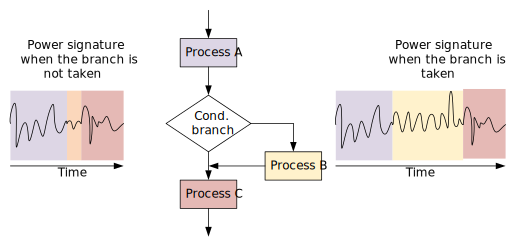
\includegraphics[width=0.8\textwidth,height=\textheight]{img/side_channel_leakage_figure_1_branch.pdf}
\caption{leakage of conditional branch}
\end{figure}

Cycle timing resulting from specific data values -- The execution cycles
of some instructions can be dependent on the values of input data,
resulting in timing side-channel leakage. E.g., the integer divide
instruction in Arm Cortex-M processors.

\begin{figure}
\centering
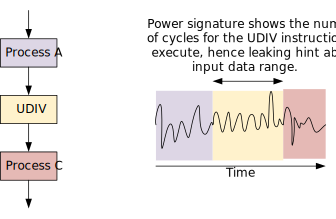
\includegraphics[width=0.8\textwidth,height=\textheight]{img/side_channel_leakage_figure_2_duration.pdf}
\caption{leakage of execution cycle}
\end{figure}

Power variation due to value changes -- The power spikes in the power
signature are often dependent on a combination of how many bits are set
and how many bits have toggled in the register(s) --- the so-called
Hamming weight and Hamming distance, so the amplitude of the spike could
be used to guess the register value in that clock cycle. The power
spikes can be caused by a combination of

\begin{itemize}
\tightlist
\item
  Logic switching due to the operations of an instruction (e.g.~power
  consumed by a single cycle multiplier can be much higher than the
  power used by a Boolean logic function), and
\item
  Logic switching due to changes in data values in the register bank and
  data paths.
\end{itemize}

The switching activities are dependent on preceding and next operations.
If the power signature of the codes around a specific instruction is
recognizable, then the data value being process could be guessed.

\begin{figure}
\centering
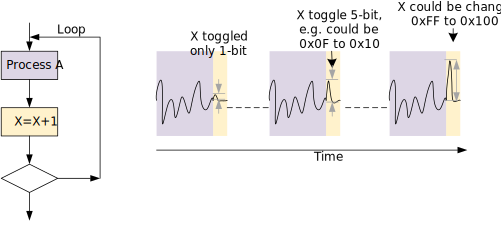
\includegraphics[width=0.8\textwidth,height=\textheight]{img/side_channel_leakage_figure_3_toggle.pdf}
\caption{leakage of number of bit toggled}
\end{figure}

In some SoC or microcontroller implementations, the power spike effect
of the operations can be much higher than the effect of data value
changes in the register banks. In such case the program execution flow
can be observed, and as a result, might also indirectly leak information
about the data that it is processing.

\hypertarget{countermeasures}{%
\subsection{Countermeasures}\label{countermeasures}}

For normal embedded devices that don't have physical protection
features, there is a much higher chance that power/voltage/radiation
side channels can result in information leakage. However, some aspects
of timing signature leakage could be reduced:

\begin{itemize}
\tightlist
\item
  Using data processing instruction with data independent timing for
  cryptographic operations. In recent Arm architectures (including
  Armv8-A and Armv8-M), some instructions are architecturally defined as
  DIT (Data Independent Timing).
\item
  For conditional branches where the condition is dependent on secret
  data, use table branch instead might help reduce timing base leakage
  (both paths result in a branch). It is not necessary to replace all
  conditional branch. For example, many loop counters in crypto
  operation can be independent to the crypto key or input data values,
  so there is no need to change those loops.
\end{itemize}

\tododiv{There is overlap with section timing-side-channels. How to best
consolidate that?
\href{https://github.com/llsoftsec/llsoftsecbook/issues/182}{\#182}}

There are additional software techniques to mitigate power leakage. One
of the most well-known techniques is masking (e.g.~Boolean,
multiplicative, affine). When applying software mitigation, software
developers need to check that optimizations carried out by compilers
(C/C++) do not impact the mitigation, as compilers can be very smart and
undo the masking in order to perform faster operations (or reducing code
size).

\hypertarget{fault-injection-attacks}{%
\section{Fault injection attacks}\label{fault-injection-attacks}}

\hypertarget{common-forms-of-fault-injection-attacks}{%
\subsection{Common forms of Fault injection
attacks}\label{common-forms-of-fault-injection-attacks}}

If an attacker has physical access to a device, they can also choose to
use physical attacks to modify the behavior of the software, for
example, prevent the software from setting up certain security features
during the device's initialization sequence. The two most common forms
of such attacks are voltage glitching and clock glitching.

\begin{figure}
\centering
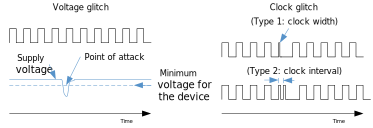
\includegraphics[width=0.8\textwidth,height=\textheight]{img/physical_attacks.pdf}
\caption{common fault injection attacks}
\end{figure}

\begin{itemize}
\tightlist
\item
  Voltage glitch attack

  \begin{itemize}
  \tightlist
  \item
    Using a programmable power supply that can switch the voltage level
    rapidly, it is possible to reduce/increase the power supply voltage
    of a chip at specific clock cycle of the software execution. In some
    case, a precise voltage drop can cause a processor to ``skip'' an
    instruction, for example, the write to memory or a hardware register
    might not be taken. Or if a write has taken place, the actual write
    value used could be changed by the voltage glitch.
  \end{itemize}
\item
  Clock glitch attack

  \begin{itemize}
  \tightlist
  \item
    Using a clock switching circuit, it is possible to reduce the width
    of a clock pulse, or the interval between two clock pulses so that
    some of the hardware registers are not updated correctly at certain
    clock edge(s). Similar to voltage glitch, this can make the hardware
    seems to be skipping an instruction.
  \end{itemize}
\end{itemize}

Such voltage/clock glitch attack could affect multiple parts in the
processors, but sometimes the impact might not lead to any visible error
in the operation, leaving the only effect that the processor skipping a
memory/register write, or writing an incorrect value. Potentially, a
glitch attack could result in other observable effect (e.g.~register
reset, bit toggle). The analysis of fault injection methods (and their
physical effect) and the observable effects at the program or
instruction execution level are often referred to as fault models, where
one can say that a specific fault injection behaves as an instruction
skip, etc. More details about the concept of fault models can be found
in the paper \href{https://arxiv.org/pdf/2003.10513.pdf}{``Fault Attacks
on Secure Embedded Software: Threats, Design and Evaluation''}, where a
good illustration of the concept is shown in figure 1 of that paper.

\tododiv{Make the above reference to a paper use bibtex.
\href{https://github.com/llsoftsec/llsoftsecbook/issues/159}{\#159}}

Using glitching methods, there are several common ways of attacking a
system. For example:

\begin{itemize}
\tightlist
\item
  Skipping an instruction during setup sequence for security features --
  e.g. skipping the write to the MPU (Memory Protection Unit)/Security
  Attribution Unit (SAU) so that the MPU/SAU is not enabled.
\item
  Skipping an instruction after a security authentication that branch to
  an error handling code. As the branch is not taken, the code can
  continue to operate even a security authentication has failed.
\item
  Causing an incorrect value to be written in a memory or hardware. E.g.
  When writing a crypto key to a crypto accelerator, forcing the key
  value written to be zero (caused to low voltage on bus hardware).
\end{itemize}

Example: \href{https://www.youtube.com/watch?v=4u6BAH8mEDw}{Attack on
TrustZone for Armv8-M}

There are other forms of physical attacks, but most of them requires
significant effort or cost (e.g.~cut open the chip package can carry out
fault injection or readout secret data on chip).

\hypertarget{countermeasures-1}{%
\subsection{Countermeasures}\label{countermeasures-1}}

Ideally, system designers can use hardware (SoCs or microcontroller)
that support protection against fault injection. For example, a hardware
circuit can include redundancy logic (spatial and temporal). In
addition, software developers can make such attack harder by adding
checks after the write operations. When applying software mitigation,
software developers need to check that optimizations carried out by
compilers (C/C++) do not impact the mitigation.

\hypertarget{other-security-topics-relevant-for-compiler-developers}{%
\chapter{Other security topics relevant for compiler
developers}\label{other-security-topics-relevant-for-compiler-developers}}

\tododiv{Write chapter with other security topics.}

\hypertarget{appendix-contribution-guidelines}{%
\chapter*{Appendix: contribution
guidelines}\label{appendix-contribution-guidelines}}
\addcontentsline{toc}{chapter}{Appendix: contribution guidelines}

If you'd like to start contributing to this book: please do, we're
looking forward to your contributions!

The project lives on github at
\url{https://github.com/llsoftsec/llsoftsecbook}. We also have a Discord
server where you can have an interactive chat with us at
\url{https://discord.gg/Bm55Z9Ppgn}.

We use \href{https://github.com/llsoftsec/llsoftsecbook/issues}{github
issues} as our issue tracker and use
\href{https://github.com/llsoftsec/llsoftsecbook/pulls}{github pull
requests} to accept edits, changes, additions and more.

If you'd like to contribute, but are not sure where to start, the list
of open issues labeled with
``\href{https://github.com/llsoftsec/llsoftsecbook/issues?q=is\%3Aissue+is\%3Aopen+label\%3A\%22good+first+issue\%22}{good
first issue}'' may give you inspiration of things to contribute. Please,
also don't be shy to reach out to us on
\href{https://discord.gg/Bm55Z9Ppgn}{Discord}.

We follow the
\href{https://github.com/llsoftsec/llsoftsecbook/blob/main/CODE_OF_CONDUCT.md}{Contributor
Covenant Code of Conduct} in this project.

For more details on how to write text for the book, please read
\href{https://github.com/llsoftsec/llsoftsecbook/blob/main/contributing.md}{contributing.md}.
If after reading that, you think some specific aspects could be
explained better, please do let us know by raising an
\href{https://github.com/llsoftsec/llsoftsecbook/issues/new}{issue}.

\printindex

\hypertarget{references}{%
\chapter*{References}\label{references}}
\addcontentsline{toc}{chapter}{References}

\hypertarget{refs}{}
\begin{CSLReferences}{1}{0}
\leavevmode\vadjust pre{\hypertarget{ref-GNUMemSet}{}}%
{``10.604 Memset\_explicit.''} n.d.
\url{https://www.gnu.org/software//gnulib/manual/html_node/memset_005fexplicit.html}.

\leavevmode\vadjust pre{\hypertarget{ref-Aciicmez2007}{}}%
Aciiçmez, Onur, Çetin Kaya Koç, and Jean-Pierre Seifert. 2007. {``On the
Power of Simple Branch Prediction Analysis.''} In \emph{Proceedings of
the 2nd {ACM} Symposium on Information, Computer and Communications
Security}. {ACM}. \url{https://doi.org/10.1145/1229285.1266999}.

\leavevmode\vadjust pre{\hypertarget{ref-AlephOne1996}{}}%
Aleph One. 1996. {``Smashing the Stack for Fun and Profit.''} 1996.
\url{http://www.phrack.org/issues/49/14.html\#article}.

\leavevmode\vadjust pre{\hypertarget{ref-pep572}{}}%
Angelico, Chris, Tim Peters, and Guido van Rossum. 2018. {``Assignment
Expressions.''} PEP 572. \url{https://peps.python.org/pep-0572/}.

\leavevmode\vadjust pre{\hypertarget{ref-Beer2020}{}}%
Beer, Ian. 2020. {``An iOS Zero-Click Radio Proximity Exploit
Odyssey.''} 2020.
\url{https://googleprojectzero.blogspot.com/2020/12/an-ios-zero-click-radio-proximity.html}.

\leavevmode\vadjust pre{\hypertarget{ref-Beer2021}{}}%
Beer, Ian, and Samuel Groß. 2021. {``A Deep Dive into an NSO Zero-Click
iMessage Exploit: Remote Code Execution.''} 2021.
\url{https://googleprojectzero.blogspot.com/2021/12/a-deep-dive-into-nso-zero-click.html}.

\leavevmode\vadjust pre{\hypertarget{ref-Bletsch2011}{}}%
Bletsch, Tyler, Xuxian Jiang, Vince W. Freeh, and Zhenkai Liang. 2011.
{``Jump-Oriented Programming: A New Class of Code-Reuse Attack.''} In
\emph{Proceedings of the 6th ACM Symposium on Information, Computer and
Communications Security}, 30--40. ASIACCS '11. New York, NY, USA:
Association for Computing Machinery.
\url{https://doi.org/10.1145/1966913.1966919}.

\leavevmode\vadjust pre{\hypertarget{ref-Bosman2014}{}}%
Bosman, Erik, and Herbert Bos. 2014. {``Framing Signals - a Return to
Portable Shellcode.''} In \emph{2014 IEEE Symposium on Security and
Privacy}, 243--58. \url{https://doi.org/10.1109/SP.2014.23}.

\leavevmode\vadjust pre{\hypertarget{ref-Boucher2023}{}}%
Boucher, Nicholas, and Ross Anderson. 2023. {``Trojan Source: Invisible
Vulnerabilities.''} In \emph{32nd USENIX Security Symposium (USENIX
Security 23)}. Anaheim, CA: USENIX Association.
\url{https://arxiv.org/abs/2111.00169}.

\leavevmode\vadjust pre{\hypertarget{ref-Briongos2020}{}}%
Briongos, Samira, Pedro Malagon, Jose M. Moya, and Thomas Eisenbarth.
2020. {``{RELOAD+REFRESH}: Abusing Cache Replacement Policies to Perform
Stealthy Cache Attacks.''} In \emph{29th USENIX Security Symposium
(USENIX Security 20)}.
\url{https://www.usenix.org/conference/usenixsecurity20/presentation/briongos}.

\leavevmode\vadjust pre{\hypertarget{ref-Bulck2020}{}}%
Bulck, Jo Van, Daniel Moghimi, Michael Schwarz, Moritz Lippi, Marina
Minkin, Daniel Genkin, Yuval Yarom, Berk Sunar, Daniel Gruss, and Frank
Piessens. n.d. {``{LVI}: Hijacking Transient Execution Through
Microarchitectural Load Value Injection.''} In \emph{2020 {IEEE}
Symposium on Security and Privacy ({SP})}.

\leavevmode\vadjust pre{\hypertarget{ref-Bulygin2008}{}}%
Bulygin, Yuriy. 2008. {``{CPU} Side-Channels Vs. Virtualization
Rootkits: The Good, the Bad, or the Ugly.''} In \emph{CPU Side-Channels
Vs. Virtualization Rootkits: The Good, the Bad, or the Ugly}.
\url{https://infocondb.org/con/toorcon/toorcon-seattle-2008/cpu-side-channels-vs-virtualization-rootkits-the-good-the-bad-or-the-ugly}.

\leavevmode\vadjust pre{\hypertarget{ref-Burow2017}{}}%
Burow, Nathan, Scott A. Carr, Joseph Nash, Per Larsen, Michael Franz,
Stefan Brunthaler, and Mathias Payer. 2017. {``Control-Flow Integrity:
Precision, Security, and Performance.''} \emph{ACM Comput. Surv.} 50
(1). \url{https://doi.org/10.1145/3054924}.

\leavevmode\vadjust pre{\hypertarget{ref-Chen2005}{}}%
Chen, Shuo, Jun Xu, Emre Can Sezer, Prachi Gauriar, and Ravishankar K
Iyer. 2005. {``Non-Control-Data Attacks Are Realistic Threats.''} In
\emph{USENIX Security Symposium}, 5:146.

\leavevmode\vadjust pre{\hypertarget{ref-Conti2015}{}}%
Conti, Mauro, Stephen Crane, Lucas Davi, Michael Franz, Per Larsen,
Marco Negro, Christopher Liebchen, Mohaned Qunaibit, and Ahmad-Reza
Sadeghi. 2015. {``Losing Control: On the Effectiveness of Control-Flow
Integrity Under Stack Attacks.''} In \emph{Proceedings of the 22nd ACM
SIGSAC Conference on Computer and Communications Security}, 952--63. CCS
'15. New York, NY, USA: Association for Computing Machinery.
\url{https://doi.org/10.1145/2810103.2813671}.

\leavevmode\vadjust pre{\hypertarget{ref-Cook2023}{}}%
Cook, Kees. 2023. {``Bounded Flexible Arrays in {C}.''} 2023.
\url{https://people.kernel.org/kees/bounded-flexible-arrays-in-c}.

\leavevmode\vadjust pre{\hypertarget{ref-Cox2015}{}}%
Cox, Joseph. 2015. {``Hack Brief: Malware Sneaks into the Chinese iOS
App Store.''} \emph{WIRED}.
\url{https://www.wired.com/2015/09/hack-brief-malware-sneaks-chinese-ios-app-store/}.

\leavevmode\vadjust pre{\hypertarget{ref-d2015correctness}{}}%
D'Silva, Vijay, Mathias Payer, and Dawn Song. 2015. {``The
Correctness-Security Gap in Compiler Optimization.''} In \emph{2015 IEEE
Security and Privacy Workshops}, 73--87. IEEE.

\leavevmode\vadjust pre{\hypertarget{ref-Dowd2006}{}}%
Dowd, Mark, John McDonald, and Justin Schuh. 2006. \emph{The Art of
Software Security Assessment: Identifying and Preventing Software
Vulnerabilities}. Addison-Wesley Professional.

\leavevmode\vadjust pre{\hypertarget{ref-dusilent}{}}%
Du, Jianhao Xu1 Kangjie Lu2 Zhengjie, Zhu Ding1 Linke Li1 Qiushi Wu, and
Mathias Payer3 Bing Mao. n.d. {``Silent Bugs Matter: A Study of
Compiler-Introduced Security Bugs.''}

\leavevmode\vadjust pre{\hypertarget{ref-Dullien2020}{}}%
Dullien, Thomas. 2020. {``Weird Machines, Exploitability, and Provable
Unexploitability.''} \emph{IEEE Transactions on Emerging Topics in
Computing} 8 (2): 391--403.
\url{https://doi.org/10.1109/TETC.2017.2785299}.

\leavevmode\vadjust pre{\hypertarget{ref-Evtyushkin2018}{}}%
Evtyushkin, Dmitry, Ryan Riley, Nael CSE, ECE Abu-Ghazaleh, and Dmitry
Ponomarev. 2018. {``BranchScope: A New Side-Channel Attack on
Directional Branch Predictor.''} In \emph{Proceedings of the
Twenty-Third International Conference on Architectural Support for
Programming Languages and Operating Systems}.
\url{https://doi.org/10.1145/3173162.3173204}.

\leavevmode\vadjust pre{\hypertarget{ref-Eyerman2009}{}}%
Eyerman, Stijn, Lieven Eeckhout, Tejas Karkhanis, and James E. Smith.
2009. {``A Mechanistic Performance Model for Superscalar Out-of-Order
Processors.''} \emph{{ACM} Transactions on Computer Systems} 27 (2).
\url{https://doi.org/10.1145/1534909.1534910}.

\leavevmode\vadjust pre{\hypertarget{ref-Fetiveau2019}{}}%
Fetiveau, Jeremy. 2019. {``Circumventing Chrome's Hardening of Typer
Bugs.''} 2019.
\url{https://doar-e.github.io/blog/2019/05/09/circumventing-chromes-hardening-of-typer-bugs/}.

\leavevmode\vadjust pre{\hypertarget{ref-Dullien2018}{}}%
Flake, Thomas Dullien/Halvar. 2018. {``Turing Completeness, Weird
Machines, Twitter, and Muddled Terminology.''} 2018.
\url{http://addxorrol.blogspot.com/2018/10/turing-completeness-weird-machines.html}.

\leavevmode\vadjust pre{\hypertarget{ref-FbsdJunk}{}}%
{``FreeBSD Mitigation for Srandom Undefined Behavior.''} 2012. 2012.
\url{https://github.com/freebsd/freebsd-src/commit/6a762eb23ea5f31e65cfa12602937f39a14e9b0c}.

\leavevmode\vadjust pre{\hypertarget{ref-MozillaIssue}{}}%
{``GCC6 - TB Crashes Due to Removed Null Pointer Checks for "This".''}
2016. 2016. \url{https://bugzilla.mozilla.org/show_bug.cgi?id=1251576}.

\leavevmode\vadjust pre{\hypertarget{ref-Glazunov2021}{}}%
Glazunov, Sergei. 2021. {``In-the-Wild Series: Chrome Infinity Bug.''}
2021.
\url{https://googleprojectzero.blogspot.com/2021/01/in-wild-series-chrome-infinity-bug.html}.

\leavevmode\vadjust pre{\hypertarget{ref-Gostev2009}{}}%
Gostev, Alexander. 2009. {``A Short History of Induc.''} 2009.
\url{https://securelist.com/a-short-history-of-induc/30555/}.

\leavevmode\vadjust pre{\hypertarget{ref-Greenberg2019}{}}%
Greenberg, Andy. 2019. {``Supply Chain Hackers Snuck Malware into
Videogames.''} \emph{WIRED}.
\url{https://www.wired.com/story/supply-chain-hackers-videogames-asus-ccleaner/}.

\leavevmode\vadjust pre{\hypertarget{ref-Grouxdf2020}{}}%
Groß, Samuel. 2020. {``JITSploitation i: A JIT Bug.''} 2020.
\url{https://googleprojectzero.blogspot.com/2020/09/jitsploitation-one.html}.

\leavevmode\vadjust pre{\hypertarget{ref-Grouxdf2022}{}}%
Groß, Samuel, and Amy Burnett. 2022. {``Attacking JavaScript Engines in
2022.''} 2022.
\url{https://saelo.github.io/presentations/offensivecon_22_attacking_javascript_engines.pdf}.

\leavevmode\vadjust pre{\hypertarget{ref-Gruss2016}{}}%
Gruss, Daniel, Clémentine Maurice, Anders Fogh, Moritz Lipp, and Stefan
Mangard. 2016. {``Prefetch Side-Channel Attacks: Bypassing SMAP and
Kernel ASLR.''} In \emph{Proceedings of the 2016 ACM SIGSAC Conference
on Computer and Communications Security}. CCS '16.
\url{https://doi.org/10.1145/2976749.2978356}.

\leavevmode\vadjust pre{\hypertarget{ref-Gruss2016a}{}}%
Gruss, Daniel, Clémentine Maurice, Klaus Wagner, and Stefan Mangard.
2016. {``Flush+flush: A Fast and Stealthy Cache Attack.''} In
\emph{Proceedings of the 13th International Conference on Detection of
Intrusions and Malware, and Vulnerability Assessment - Volume 9721},
279--99. DIMVA 2016. \url{https://doi.org/10.1007/978-3-319-40667-1_14}.

\leavevmode\vadjust pre{\hypertarget{ref-Hicks2014}{}}%
Hicks, Michael. 2014. {``What Is Memory Safety?''} 2014.
\url{http://www.pl-enthusiast.net/2014/07/21/memory-safety/}.

\leavevmode\vadjust pre{\hypertarget{ref-Hu2016}{}}%
Hu, Hong, Shweta Shinde, Sendroiu Adrian, Zheng Leong Chua, Prateek
Saxena, and Zhenkai Liang. 2016. {``Data-Oriented Programming: On the
Expressiveness of Non-Control Data Attacks.''} In \emph{2016 IEEE
Symposium on Security and Privacy (SP)}, 969--86.
\url{https://doi.org/10.1109/SP.2016.62}.

\leavevmode\vadjust pre{\hypertarget{ref-Huo2019}{}}%
Huo, Tianlin, Xiaoni Meng, Wenhao Wang, Chunliang Hao, Pei Zhao, Jian
Zhai, and Mingshu Li. 2019. {``Bluethunder: A 2-Level Directional
Predictor Based Side-Channel Attack Against {SGX}.''} \emph{{IACR}
Transactions on Cryptographic Hardware and Embedded Systems}, November.
\url{https://doi.org/10.46586/tches.v2020.i1.321-347}.

\leavevmode\vadjust pre{\hypertarget{ref-Ispoglou2018}{}}%
Ispoglou, Kyriakos K., Bader AlBassam, Trent Jaeger, and Mathias Payer.
2018. {``Block Oriented Programming: Automating Data-Only Attacks.''} In
\emph{Proceedings of the 2018 ACM SIGSAC Conference on Computer and
Communications Security}, 1868--82. CCS '18. New York, NY, USA:
Association for Computing Machinery.
\url{https://doi.org/10.1145/3243734.3243739}.

\leavevmode\vadjust pre{\hypertarget{ref-ChromiumIssue}{}}%
{``Issue 3782: V8 Is Not -Fsanitize=null Clean.''} 2014. 2014.
\url{https://bugs.chromium.org/p/v8/issues/detail?id=3782}.

\leavevmode\vadjust pre{\hypertarget{ref-Kocher2019}{}}%
Kocher, Paul, Jann Horn, Anders Fogh, Daniel Genkin, Daniel Gruss,
Werner Haas, Mike Hamburg, et al. 2019. {``Spectre Attacks: Exploiting
Speculative Execution.''} In \emph{2019 {IEEE} Symposium on Security and
Privacy ({SP})}. {IEEE}. \url{https://doi.org/10.1109/sp.2019.00002}.

\leavevmode\vadjust pre{\hypertarget{ref-Lee2017}{}}%
Lee, Sangho, Ming-Wei Shih, Prasun Gera, Taesoo Kim, Hyesoon Kim, and
Marcus Peinado. 2017. {``Inferring Fine-Grained Control Flow Inside
{SGX} Enclaves with Branch Shadowing.''} In \emph{26th USENIX Security
Symposium (USENIX Security 17)}.
\url{https://www.usenix.org/conference/usenixsecurity17/technical-sessions/presentation/lee-sangho}.

\leavevmode\vadjust pre{\hypertarget{ref-MemZeroDataBarrier}{}}%
{``Lib: Make Memzero\_explicit More Robust Against Dead Store
Elimination.''} 2015. 2015.
\url{https://github.com/torvalds/linux/commit/7829fb09a2b4268b30dd9bc782fa5ebee278b137}.

\leavevmode\vadjust pre{\hypertarget{ref-OpenSSLMemClr}{}}%
---------. 2016. 2016.
\url{https://github.com/openssl/openssl/commit/104ce8a9f02d250dd43c255eb7b8747e81b29422}.

\leavevmode\vadjust pre{\hypertarget{ref-MemZeroBarrier}{}}%
{``Lib: Memzero\_explicit: Use Barrier Instead of
{OPTIMIZER\_HIDE\_VAR}.''} 2015. 2015.
\url{https://github.com/torvalds/linux/commit/0b053c9518292705736329a8fe20ef4686ffc8e9}.

\leavevmode\vadjust pre{\hypertarget{ref-Liljestrand2021}{}}%
Liljestrand, Hans, Thomas Nyman, Lachlan J Gunn, Jan-Erik Ekberg, and N
Asokan. 2021. {``\(\{\)PACStack\(\}\): An Authenticated Call Stack.''}
In \emph{30th USENIX Security Symposium (USENIX Security 21)}, 357--74.

\leavevmode\vadjust pre{\hypertarget{ref-Lipp2020}{}}%
Lipp, Moritz, Vedad Hadzic, Michael Schwarz, Arthur Perais, Clementine
Lucie Noemie Maurice, and Daniel Gruß. 2020. {``Take a Way: Exploring
the Security Implications of AMD's Cache Way Predictors.''} In
\emph{Proceedings of the 15th ACM Asia Conference on Computer and
Communications Security, ASIA CCS 2020}.
\url{https://doi.org/10.1145/3320269.3384746}.

\leavevmode\vadjust pre{\hypertarget{ref-Lipp2018}{}}%
Lipp, Moritz, Michael Schwarz, Daniel Gruss, Thomas Prescher, Werner
Haas, Anders Fogh, Jann Horn, et al. 2018. {``Meltdown: Reading Kernel
Memory from User Space.''} In \emph{27th USENIX Security Symposium
(USENIX Security 18)}.
\url{https://www.usenix.org/conference/usenixsecurity18/presentation/lipp}.

\leavevmode\vadjust pre{\hypertarget{ref-McCall2019}{}}%
McCall, John, and Ahmed Bougacha. 2019. {``Arm64e: An ABI for Pointer
Authentication.''} 2019.
\url{https://llvm.org/devmtg/2019-10/slides/McCall-Bougacha-arm64e.pdf}.

\leavevmode\vadjust pre{\hypertarget{ref-MemSetProposal}{}}%
{``Memset\_explicit.''} 2021. 2021.
\url{https://www.open-std.org/jtc1/sc22/wg14/www/docs/n2897.htm}.

\leavevmode\vadjust pre{\hypertarget{ref-Miller2012}{}}%
Miller, Matt. n.d. {``Modeling the Exploitation and Mitigation of Memory
Safety Vulnerabilities.''}
\href{https://2012.ruxconbreakpoint.com/}{Breakpoint 2012}.
\url{https://github.com/Microsoft/MSRC-Security-Research/blob/master/presentations/2012_10_Breakpoint/BreakPoint2012_Miller_Modeling_the_exploitation_and_mitigation_of_memory_safety_vulnerabilities.pdf}.

\leavevmode\vadjust pre{\hypertarget{ref-Mushtaq2020}{}}%
Mushtaq, Maria, Muhammad Asim Mukhtar, Vianney Lapotre, Muhammad Khurram
Bhatti, and Guy Gogniat. 2020. {``Winter Is Here! A Decade of
Cache-Based Side-Channel Attacks, Detection \& Mitigation for {RSA}.''}
\emph{Information Systems}, September.
\url{https://doi.org/10.1016/j.is.2020.101524}.

\leavevmode\vadjust pre{\hypertarget{ref-Mutlu2004}{}}%
Mutlu, Onur, Hyesoon Kim, David N. Armstrong, and Yale N. Patt. 2004.
{``Understanding the Effects of Wrong-Path Memory References on
Processor Performance.''} In \emph{Proceedings of the 3rd Workshop on
Memory Performance Issues in Conjunction with the 31st International
Symposium on Computer Architecture - WMPI '04}.
\url{https://doi.org/10.1145/1054943.1054951}.

\leavevmode\vadjust pre{\hypertarget{ref-ObsdJunk}{}}%
{``OpenBSD Mitigation for Srandom Undefined Behavior.''} 2002. 2002.
\url{https://github.com/openbsd/src/commit/99d815f892ce481695caf21f08f773f563820a66}.

\leavevmode\vadjust pre{\hypertarget{ref-Osvik2005}{}}%
Osvik, Dag Arne, Adi Shamir, and Eran Tromer. 2005. {``Cache Attacks and
Countermeasures: The Case of AES.''} In \emph{IACR Cryptology ePrint
Archive}. \url{https://doi.org/10.1007/11605805_1}.

\leavevmode\vadjust pre{\hypertarget{ref-Karger1974}{}}%
Paul A., Karger, and Schell Roger R. 1974. {``MULTICS SECURITY
EVALUATION: VULNERABILITY ANALYSIS,''} 52.
\url{https://csrc.nist.gov/csrc/media/publications/conference-paper/1998/10/08/proceedings-of-the-21st-nissc-1998/documents/early-cs-papers/karg74.pdf}.

\leavevmode\vadjust pre{\hypertarget{ref-Percival2005}{}}%
Percival, Colin. 2005. {``Cache Missing for Fun and Profit.''} BSDCan.
\url{https://eprint.iacr.org/2005/271}.

\leavevmode\vadjust pre{\hypertarget{ref-Pizlo2020}{}}%
Pizlo, Filip. 2020. {``Speculation in JavaScriptCore.''} 2020.
\url{https://webkit.org/blog/10308/speculation-in-javascriptcore/}.

\leavevmode\vadjust pre{\hypertarget{ref-Pornin2018}{}}%
Pornin, Thomas. 2018. {``Why Constant-Time Crypto?''} 2018.
\url{https://www.bearssl.org/constanttime.html}.

\leavevmode\vadjust pre{\hypertarget{ref-Rutland2017}{}}%
Rutland, Mark. 2017. {``ARMv8.3 Pointer Authentication.''} 2017.
\url{https://events.static.linuxfound.org/sites/events/files/slides/slides_23.pdf}.

\leavevmode\vadjust pre{\hypertarget{ref-saelo2021b}{}}%
saelo. 2021a. {``Attacking JavaScript Engines: A Case Study of
JavaScriptCore and CVE-2016-4622.''} 2021.
\url{http://www.phrack.org/issues/70/3.html}.

\leavevmode\vadjust pre{\hypertarget{ref-saelo2021a}{}}%
---------. 2021b. {``Exploiting Logic Bugs in JavaScript JIT Engines.''}
2021. \url{http://www.phrack.org/issues/70/9.html}.

\leavevmode\vadjust pre{\hypertarget{ref-Schuster2015}{}}%
Schuster, F., T. Tendyck, C. Liebchen, L. Davi, A. Sadeghi, and T. Holz.
2015. {``Counterfeit Object-Oriented Programming: On the Difficulty of
Preventing Code Reuse Attacks in c++ Applications.''} In \emph{2015 IEEE
Symposium on Security and Privacy (SP)}, 745--62. Los Alamitos, CA, USA:
IEEE Computer Society. \url{https://doi.org/10.1109/SP.2015.51}.

\leavevmode\vadjust pre{\hypertarget{ref-Schwarz2017}{}}%
Schwarz, Michael, Clémentine Maurice, Daniel Gruss, and Stefan Mangard.
2017. {``Fantastic Timers and Where to Find Them: High-Resolution
Microarchitectural Attacks in {JavaScript}.''} In \emph{Financial
Cryptography and Data Security}, 247--67. Springer International
Publishing.

\leavevmode\vadjust pre{\hypertarget{ref-Schwarz2019}{}}%
Schwarz, Michael, Martin Schwarzl, Moritz Lipp, Jon Masters, and Daniel
Gruss. 2019. {``NetSpectre: Read Arbitrary Memory over Network.''} In
\emph{Computer Security - {ESORICS} 2019 - 24th European Symposium on
Research in Computer Security, Luxembourg, September 23-27, 2019,
Proceedings, Part {I}}, 11735:279--99. Lecture Notes in Computer
Science. Springer.

\leavevmode\vadjust pre{\hypertarget{ref-Seacord2013}{}}%
Seacord, Robert C. 2013. \emph{Secure Coding in c and c++}. 2nd ed.
Addison-Wesley Professional.

\leavevmode\vadjust pre{\hypertarget{ref-Serebryany2012}{}}%
Serebryany, Konstantin, Derek Bruening, Alexander Potapenko, and Dmitriy
Vyukov. 2012. {``\(\{\)AddressSanitizer\(\}\): A Fast Address Sanity
Checker.''} In \emph{2012 USENIX Annual Technical Conference (USENIX ATC
12)}, 309--18.

\leavevmode\vadjust pre{\hypertarget{ref-Serna2012}{}}%
Serna, Fermin J. 2012. {``The Info Leak Era on Software Exploitation.''}
2012. \url{https://www.youtube.com/watch?v=VgWoPa8Whmc}.

\leavevmode\vadjust pre{\hypertarget{ref-Shacham2007}{}}%
Shacham, Hovav. 2007. {``The Geometry of Innocent Flesh on the Bone:
Return-into-Libc Without Function Calls (on the X86).''} In
\emph{Proceedings of the 14th ACM Conference on Computer and
Communications Security}, 552--61. CCS '07. New York, NY, USA:
Association for Computing Machinery.
\url{https://doi.org/10.1145/1315245.1315313}.

\leavevmode\vadjust pre{\hypertarget{ref-Sharma2014}{}}%
Sharma, Siddharth. 2014. {``Enhance Application Security with
FORTIFY\_SOURCE.''} 2014.
\url{https://www.redhat.com/en/blog/enhance-application-security-fortifysource}.

\leavevmode\vadjust pre{\hypertarget{ref-Soares2021}{}}%
Soares, Luigi, and Fernando Magno Quintan Pereira. 2021. {``Memory-Safe
Elimination of Side Channels.''} In \emph{2021 {IEEE}/{ACM}
International Symposium on Code Generation and Optimization ({CGO})}.
{IEEE}. \url{https://doi.org/10.1109/cgo51591.2021.9370305}.

\leavevmode\vadjust pre{\hypertarget{ref-Solar1997}{}}%
Solar Designer. 1997. {``Getting Around Non-Executable Stack (and
Fix).''} 1997. \url{https://seclists.org/bugtraq/1997/Aug/63}.

\leavevmode\vadjust pre{\hypertarget{ref-Song2015}{}}%
Song, Chengyu, Chao Zhang, Tielei Wang, Wenke Lee, and David Melski.
2015. {``Exploiting and Protecting Dynamic Code Generation.''} In
\emph{NDSS}.

\leavevmode\vadjust pre{\hypertarget{ref-Su2021}{}}%
Su, Chao, and Qingkai Zeng. 2021. {``Survey of {CPU} Cache-Based
Side-Channel Attacks: Systematic Analysis, Security Models, and
Countermeasures.''} \emph{Security and Communication Networks}, June.
\url{https://doi.org/10.1155/2021/5559552}.

\leavevmode\vadjust pre{\hypertarget{ref-Thompson1984}{}}%
Thompson, Ken. 1984. {``Reflections on Trusting Trust.''}
\url{https://www.cs.cmu.edu/~rdriley/487/papers/Thompson_1984_ReflectionsonTrustingTrust.pdf}.

\leavevmode\vadjust pre{\hypertarget{ref-Wang2015}{}}%
Wang, Xi. 2015. {``More Randomness or Less.''} 2015.
\url{https://kqueue.org/blog/2012/06/25/more-randomness-or-less/}.

\leavevmode\vadjust pre{\hypertarget{ref-wang2012undefined}{}}%
Wang, Xi, Haogang Chen, Alvin Cheung, Zhihao Jia, Nickolai Zeldovich,
and M Frans Kaashoek. 2012. {``Undefined Behavior: What Happened to My
Code?''} In \emph{Proceedings of the Asia-Pacific Workshop on Systems},
1--7.

\leavevmode\vadjust pre{\hypertarget{ref-Weber2021}{}}%
Weber, Daniel, Ahmad Ibrahim, Hamed Nemati, Michael Schwarz, and
Christian Rossow. 2021. {``Osiris: Automated Discovery of
Microarchitectural Side Channels.''} In \emph{USENIX Security'21}.
\url{https://arxiv.org/abs/2106.03470}.

\leavevmode\vadjust pre{\hypertarget{ref-Wheeler2020}{}}%
Wheeler, David A. 2020. {``Initial Analysis of Underhanded Source
Code.''} Institute for Defense Analyses.
\url{https://www.ida.org/research-and-publications/publications/all/i/in/initial-analysis-of-underhanded-source-code}.

\leavevmode\vadjust pre{\hypertarget{ref-Wingo2011}{}}%
Wingo, Any. 2011. {``Value Representation in JavaScript
Implementations.''} 2011.
\url{https://wingolog.org/archives/2011/05/18/value-representation-in-javascript-implementations}.

\leavevmode\vadjust pre{\hypertarget{ref-Wu2018}{}}%
Wu, Meng, Shengjian Guo, Patrick Schaumont, and Chao Wang. 2018.
{``Eliminating Timing Side-Channel Leaks Using Program Repair.''} In
\emph{Proceedings of the 27th {ACM} {SIGSOFT} International Symposium on
Software Testing and Analysis}. {ACM}.
\url{https://doi.org/10.1145/3213846.3213851}.

\leavevmode\vadjust pre{\hypertarget{ref-Yarom2014}{}}%
Yarom, Yuval, and Katrina Falkner. 2014. {``{FLUSH+RELOAD}: A High
Resolution, Low Noise, L3 Cache {Side-Channel} Attack.''} In \emph{23rd
USENIX Security Symposium (USENIX Security 14)}, 719--32. San Diego, CA:
USENIX Association.
\url{https://www.usenix.org/conference/usenixsecurity14/technical-sessions/presentation/yarom}.

\end{CSLReferences}

\end{document}
